\chapter{Slepian Scale-Discretised Wavelets on Manifolds}\label{sec:chapter4}

\section*{Abstract}

Inspired by recent interest in geometric deep learning, this work generalises the recently developed Slepian scale-discretised wavelets on the sphere to Riemannian manifolds.
Through the sifting convolution, one may define translations and, thus, convolutions on manifolds --- which are not well-defined in general.
Slepian wavelets are constructed on a region of a manifold, and are therefore suited to problems where data only exists, or is missing in a particular region.
The Slepian functions, on which Slepian wavelets are built, are the basis functions of the Slepian spatial-spectral concentration problem.
A tiling of the Slepian harmonic line with smoothly decreasing generating functions defines the scale-discretised wavelets; allowing one to probe spatially localised, scale-dependent features of a signal.
By discretising manifolds as graphs, the Slepian functions and wavelets of a polygonal mesh are presented.
Through a wavelet transform, the wavelet coefficients of a field defined on the mesh are found and used in a straightforward thresholding denoising scheme.

\section{Introduction}

Many fields measure data which are intrinsically non-Euclidean in structure and are better modelled by manifolds or graphs.
One manifold, in particular, which is in commonplace in science and engineering is the sphere; such as in: cosmology~\cite{Bennett1996}, geophysics~\cite{Simons2006}, planetary science~\cite{Turcotte1981}, computer graphics~\cite{Ramamoorthi2004}, and signal processing~\cite{Roddy2021a}.
Often data are not observed or are missing in some region of the manifold, and hence methods which work over the whole manifold may not be appropriate.
One such example, in the spherical setting, is in cosmic microwave background analyses where foreground microwave emissions dominate the region around the  Galactic plane and are often removed~\cite{Mortlock2002}.
Wavelets are a typical approach to deal with problems of this form, which allow the probing of spatially localised, scale-dependent features of the signal.
Contamination of the wavelet coefficients at the boundaries of the region, however, still presents a problem.
Hence, to overcome this, Slepian wavelets are constructed within the region itself.

In data analyses, one often desires to extract non-trivial patterns in the data.
By projecting the data onto an appropriate basis, patterns which were not considered before may present themselves.
If one seeks to find oscillatory features, then a Fourier basis is often most appropriate, \ie{} the spherical harmonics in the spherical setting.
Wavelets, however, simultaneously extract contributions of scale-dependent features in both space and scale.
Wavelets on the sphere (\cf{} manifold) have been applied in fields such as: astrophysics and cosmology~\cite{Pen1999,Barreiro2001,Rocha2004,McEwen2004}, planetary science~\cite{Audet2011,Audet2014}, and geophysics~\cite{Loris2010,Simons2011,Simons2011b}.
Scale-discretised wavelets (on the sphere)~\cite{Wiaux2008,McEwen2018,Leistedt2013,McEwen2013,McEwen2015} lean on a tiling of the harmonic line to produce an exact wavelet transform in both the continuous and discrete settings.

A new research direction, \emph{geometric deep learning}, has evolved from an increasing interest in non-Euclidean data geometries; where convolutional networks are generalised to graph and manifold structured data (\eg{}~\cite{Bronstein2017,Perlmutter2020}).
In general, geometric learning problems are split into two categories: characterising the structure of the data, and analysing functions defined on a non-Euclidean domain.
Manifold learning models (\eg{}~\cite{Tenenbaum2000,Coifman2006b,VanDerMaaten2008}) are a set of unsupervised algorithms which capture the intrinsic structure in the data through data-driven geometries.
Moreover, signals on manifolds are increasingly prevalent in areas such as shape matching and computer graphics.
Thus, many works are emerging to generalise spectral and signal processing methods to manifolds~\cite{Coifman2006} and graphs~\cite{Shuman2013}.
In these settings, functions are supported on the manifold/the vertices of the graph, and the Fourier harmonics are the eigenfunctions of the \emph{Laplace-Beltrami operator}/eigenvectors of the \emph{graph Laplacian}.

Graphs are a fundamental data structure, which are useful in describing geometric structures of data in domains such as: social~\cite{Nettleton2013}, transportation~\cite{Mohan2014}, sensor~\cite{Kenniche2010}, and neuronal~\cite{Tang2012} networks.
Each edge in a graph is associated with a weight, which is often a measure of the similarity between two connected vertices in a graph.
The physics of the problem or the data at hand dictate which vertices are connected and their respective weights, \ie{} the weight may not necessarily be the physical distance between two vertices.
A \emph{graph signal} is a finite collection of samples with some value at each vertex at a graph.
In computer graphics, working with intrinsically geometric shapes is commonplace.
In this field, 3D shapes are often modelled as Riemannian manifolds and discretised as polygonal meshes.

It is well-known that functions cannot have finite support in the spatial and spectral domains simultaneously~\cite{Slepian1961,Slepian1983}.
In the 1960s, Slepian, Landau and Pollak solved the fundamental problem of finding and representing signals which are optimally concentrated in both domains~\cite{Slepian1961,Landau1961,Landau1962}.
The \emph{Slepian spatial-spectral concentration problem} (or the \emph{Slepian concentration problem} for short) results in the families of functions which are optimally concentrated in the spatial (spectral) domain, and exactly limited in the spectral (spatial) domain.
The Slepian concentration problem was initially formed in the Euclidean domain; however, it has since been generalised to other geometries, such as: the sphere~\cite{Simons2006,Wieczorek2005,Albertella1999,Cohen1989,Meaney1984,Daubechies1988}, and graphs~\cite{VanDeVille2017,VanDeVille2017a,Bolton2018}.
The so-called \emph{Slepian functions} arise in many fields within science and engineering, such as: medical imaging~\cite{Jackson1991}, signal processing~\cite{Mathews1985,Thomson1982}, and geophysics~\cite{Thomson1976,Simons2006a,Simons2011}.
Notably, these functions have been used in interpolation~\cite{Moore2004,Shkolnisky2006}, extrapolation~\cite{Xu1983}, inverse problems~\cite{Villiers2001,Abdelmoula2015}, and solving partial differential equations~\cite{Boyd2003,Chen2005}.

Due to recent interest in geometric deep learning, many fields are extending existing methods developed in the Euclidean domain to manifolds or graphs, \ie{}~\cite{Perlmutter2020}.
This work generalises Slepian scale-discretised wavelets on the sphere~\cite{Roddy2021a} to Riemannian manifolds.
These wavelets constitute a basis designed for incomplete data on manifolds or graphs.
Here, the scale-discretised wavelet construction on the sphere~\cite{Wiaux2008,McEwen2018,Leistedt2013,McEwen2013,McEwen2015} is extended to the Slepian domain; however, the Slepian functions are now constructed on a region of a general manifold (rather than strictly the sphere).
As before, scale-discretised wavelets exhibit an explicit inversion formula, constitute a tight frame, and have excellent localisation properties in both spectral and spatial domains.
The wavelets themselves are constructed through a tiling of the Slepian harmonic line --- built from the eigenfunctions of the Slepian concentration problem.
The wavelet transform follows through a generalisation of the \emph{sifting convolution}~\cite{Roddy2021}, which allows one to perform convolutions on (incomplete) manifolds.
The wavelet construction is analogous to the spherical case, but with the eigenfunctions of the Laplace-Beltrami operator/eigenvectors of the graph Laplacian, rather than the spherical harmonics.

Plainly, wavelets in the Slepian domain have been considered before --- this work generalises prior work on the sphere to general manifolds~\cite{Roddy2021a}.
Multiresolution analyses have been performed with prolate spheroidal wave functions~\cite{Walter2004} in the Euclidean setting.
In spherical settings, spatially localised spherical harmonic transforms are sometimes used (\eg{}~\cite{Simons1997,Wieczorek2005,Khalid2013,Khalid2013a}).
Other times, the Slepian functions on the sphere are used directly~\cite{Simons2009}.
A variety of other approaches include: established regularisation techniques based on a known singular value decomposition~\cite{Michel2017}, and wavelet-like representations without explicit inverse transforms~\cite{Simons2011}.
Extending wavelets and wavelet techniques to manifold and graph domains has been extensively reviewed (\eg{}~\cite{Dahmen1999,Coifman2006a}).

The remainder of the article is as follows.
\cref{sec:chapter4_mathematical_background_problem_formulation} presents some mathematical preliminaries of Riemannian manifolds, their representations as graphs, and polygonal meshes.
The Laplace-Beltrami operator and the graph Laplacian are then introduced.
A brief review of Slepian scale-discretised wavelets on the sphere~\cite{Roddy2021a} follows, which this works builds upon.
In \cref{sec:chapter4_working_with_manifolds} the Slepian concentration problem is adapted to the manifold setting, which results in the basis functions of a region of the manifold, \ie{} the Slepian functions.
A review of the sifting convolution~\cite{Roddy2021} follows, which allows one to perform convolutions on the (incomplete) manifold --- which are typically not well-defined.
The Slepian wavelet theory is developed in \cref{sec:chapter4_slepian_wavelets}.
Initially, the sifting convolution is expressed in the Slepian domain, which is a product in the Slepian harmonic space.
The scale-discretised framework is then introduced, followed by the generating functions which define the wavelets themselves.
The section concludes with some properties of the wavelets.
A numerical illustration is presented in \cref{sec:chapter4_numerical_illustration}, in which the Slepian functions of the head region of a polygonal mesh of Homer Simpson are computed.
A field is then placed on the mesh, and the resulting wavelets and wavelet coefficients are found.
A straightforward hard-thresholding denoising scheme is developed and performed on the Homer mesh, along with some other meshes.
A boost in signal-to-noise ratio is observed, showcasing a possible use of these wavelets.
Lastly, some concluding remarks are given in \cref{sec:chapter4_conclusions}.

\section{Mathematical Background and Problem Formulation}\label{sec:chapter4_mathematical_background_problem_formulation}

Some mathematical preliminaries are introduced in \cref{sec:chapter4_mathematical_preliminaries} with a recap of Riemannian manifolds, their representation as graphs, and polygonal meshes (a popular choice of graph).
Following this is a review of the Laplace-Beltrami operator (on manifolds) and the graph Laplacian is presented.
This work extends Slepian scale-discretised wavelets on the sphere to manifolds, a brief review of which is given in \cref{sec:chapter4_problem_formulation}.

\subsection{Mathematical Preliminaries}\label{sec:chapter4_mathematical_preliminaries}

\subsubsection{Riemannian Manifolds}

Put simply, a manifold is a space that is locally Euclidean.
For example, at a point on the surface of the Earth (\ie{} \(\twoSphere{}\)) the Earth's surface appears planar --- leading to the so-called \emph{Flat Earth} theory.
More formally, a \(d\)-dimensional manifold \(\manifold{}\) is a topological space where each point \(x\) exists in a neighbourhood that is topologically homeomorphic to a \(d\)-dimensional Euclidean space --- called the \emph{tangent space}.
Let \(\manifold{}\) denote a compact, smooth, connected \(d\)-dimensional Riemannian manifold without boundary contained in \(\mathbb{R}^{n}\).
The Hilbert space \(\hilbert{\manifold}\) is formed by the set of functions \(f : \manifold \to \mathbb{R}\) that are square-integrable with respect to the Riemannian volume \(\meshVolume{}\).
The geodesic distance between two points is denoted \(r(x,y)\), and the Laplace-Beltrami operator on \(\manifold{}\) is denoted \(\laplace{M}\).

Let \(f \in \hilbert{\manifold}\) be a real-valued function defined on a Riemannian manifold \(\manifold{}\).
The \emph{Laplace-Beltrami} operator is
%
\begin{equation}
	\laplace{M} f
	%
	= \div{\grad{f}},
\end{equation}
%
where \(\div{}\) and \(\grad{}\) are the divergence and gradient operators on the manifold \(\manifold{}\) respectively.
The Laplacian eigenproblem is defined as
%
\begin{equation}
	\laplace{M} f
	%
	= -\mu f,
\end{equation}
%
which admits an orthogonal eigensystem due to the semi-positive definiteness of the Laplace-Beltrami operator.
This eigensystem forms the square-integrable basis of the manifold \(\manifold{}\), with real eigenvalues
%
\begin{equation}
	0 \leq \mu_{1} \leq \mu_{2} \leq \ldots < \infty, % chktex 11
\end{equation}
%
and eigenfunctions \(\phi_{i}\).
A function \(f \in \hilbert{\manifold}\) can therefore be decomposed into this basis by
%
\begin{equation}
	\mesh{f}
	%
	= \sum\limits_{i} f_{i} \mesh{\phi_{i}},
\end{equation}
%
where \(f_{i}\) are the Fourier coefficients given by the usual projection onto the basis functions
%
\begin{equation}
	f_{i}
	%
	= \integrateManifold{x} \mesh{f} \mesh{\conj{\phi_{i}}}.
\end{equation}
%
In practice, one must discretise the manifolds and represent them as graphs.
A review of graphs is presented in \cref{sec:chapter4_graphs}.

\subsubsection{Graphs}\label{sec:chapter4_graphs}

For simplicity, consider a weighted undirected graph
%
\begin{equation}
	\graph
	%
	= (\vertices, \edges),
\end{equation}
%
consisting of a set of \(n\) vertices
%
\begin{equation}
	\vertices
	%
	\in \set{1,2,\ldots,n},
\end{equation}
%
and the set of edges
%
\begin{equation}
	\edges
	%
	\subseteq \vertices \times \vertices.
\end{equation}
%
A weight \(a_{i} > 0\) is associated with each vertex \(i \in \vertices\), and a weight \(w_{i j} \geq 0\) with each edge \((i,j) \in \edges\).
The Hilbert spaces \(\hilbert{\vertices}\) and \(\hilbert{\edges}\) are formed by the sets of functions \(f: \vertices \to \mathbb{R}\) and \(F: \edges \to \mathbb{R}\) respectively.
The graph gradient operator \(\grad: \hilbert{\vertices} \to \hilbert{\edges}\) is mapping of functions defined on the vertices to edges
%
\begin{equation}\label{eq:chapter4_graph_grad}
	{(\grad{f})}_{i j}
	%
	= f_{i} - f_{j}.
\end{equation}
%
The graph divergence operator \(\div: \hilbert{\edges} \to \hilbert{\vertices}\) reverses this mapping
%
\begin{equation}\label{eq:chapter4_graph_div}
	{\div{F}}_{i}
	%
	= \frac{1}{a_{i}} \sum\limits_{j : (i,j) \in \edges} w_{i j} F_{i j}.
\end{equation}

The graph Laplacian
%
\begin{equation}\label{eq:chapter4_graph_laplace}
	\laplace{G} f
	%
	= \div{\grad{f}}
\end{equation}
%
is an operator \(\laplace{G} : \hilbert{\vertices} \to \hilbert{\vertices}\).
By substituting the definitions of the gradient \cref{eq:chapter4_graph_grad} and divergence operators \cref{eq:chapter4_graph_div} on the graph into \cref{eq:chapter4_graph_laplace}
%
\begin{equation}
	{(\laplace{G} f)}_{i}
	%
	= \frac{1}{a_{i}} \sum\limits_{(i,j) \in \edges} w_{i j} (f_{i} - f_{j}).
\end{equation}

The \emph{non-normalised graph Laplacian} is defined as
%
\begin{equation}
	\laplace{G}
	%
	= \vb{K} - \vb{W},
\end{equation}
%
where \(\vb{K}\) is the degree matrix, and \(\vb{W}\) is the weight matrix.
In essence, the graph Laplacian is a difference operator for any signal \(f \in \hilbert{\graph}\)
%
\begin{equation}
	{(\laplace{G} f)}_{i}
	%
	= \sum\limits_{j \in \mathcal{n}_{i}} W_{i j} [f(i) - f(j)]
\end{equation}
%
The graph Laplacian converges to the Laplace-Beltrami operator as the number of samples goes to infinity~\cite{Belkin2007}.

\subsubsection{Polygonal Meshes}

\begin{figure}[htp]
	\centering
	\subfloat[\(\mesh{\phi_{3}}\)]
	{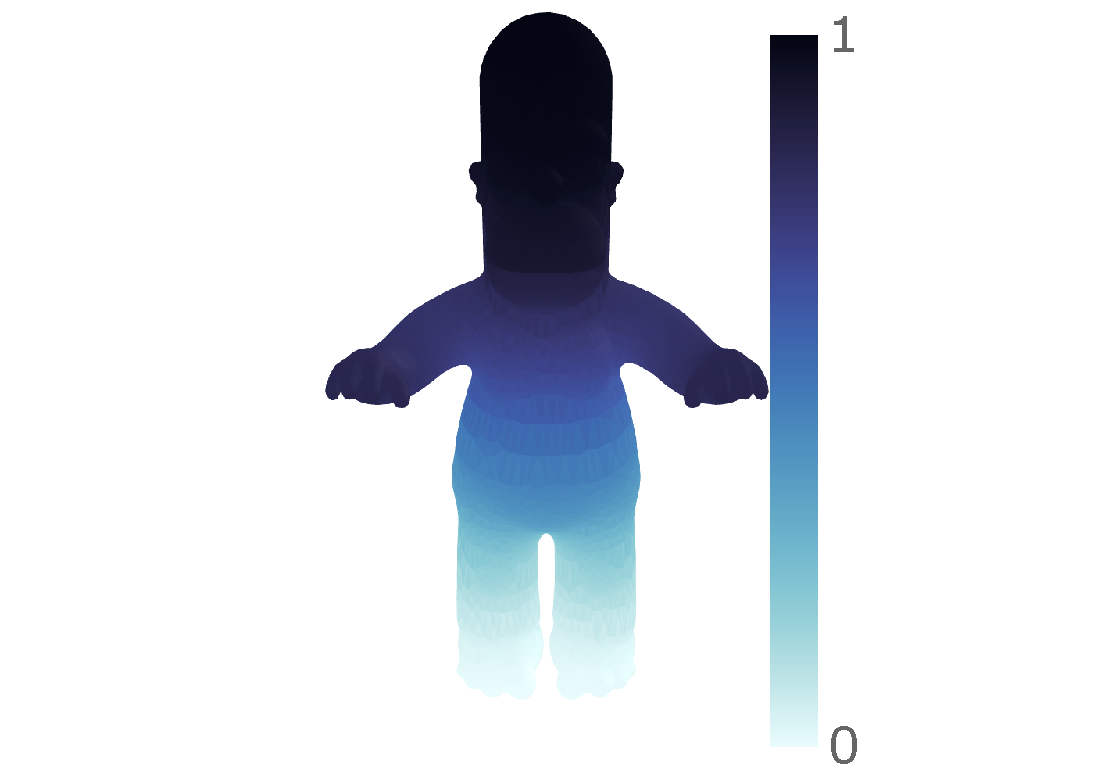
\includegraphics[trim={156 8 21 6},clip,width=.25\textwidth]{homer_rank2_lam1-325328e-03_norm.pdf}} % chktex 8
	\hfill
	\subfloat[\(\mesh{\phi_{4}}\)]
	{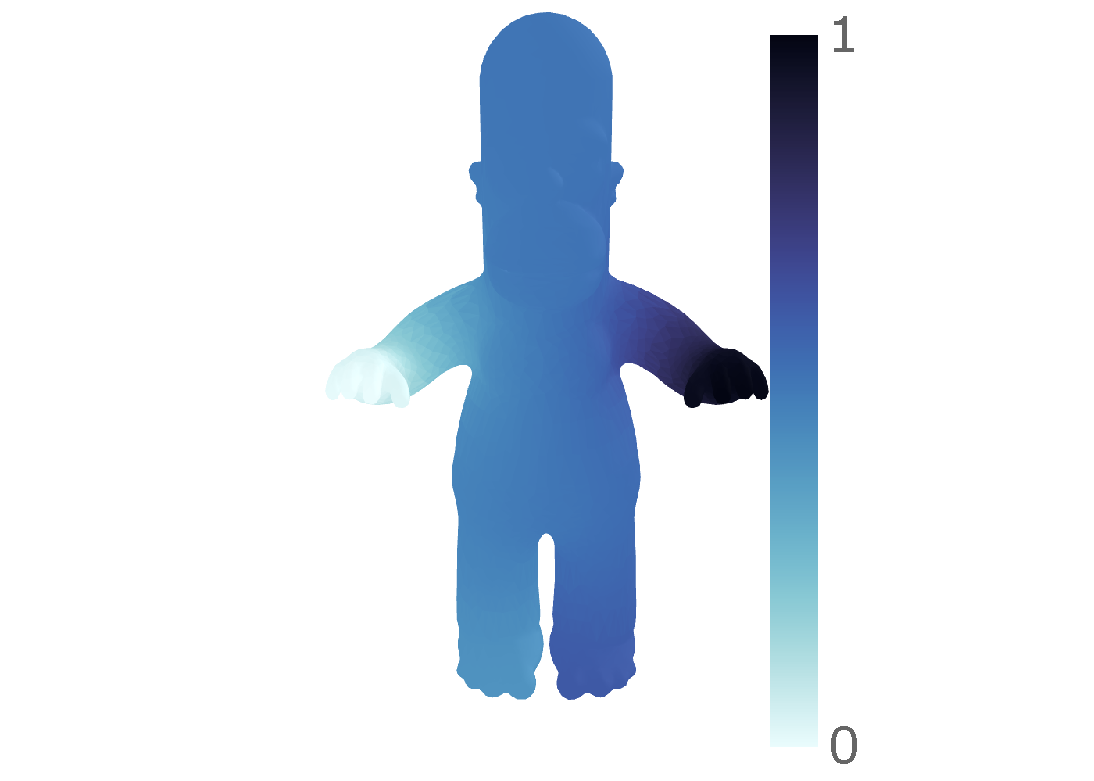
\includegraphics[trim={156 8 21 6},clip,width=.25\textwidth]{homer_rank3_lam2-425344e-03_norm.pdf}} % chktex 8
	\hfill
	\subfloat[\(\mesh{\phi_{5}}\)]
	{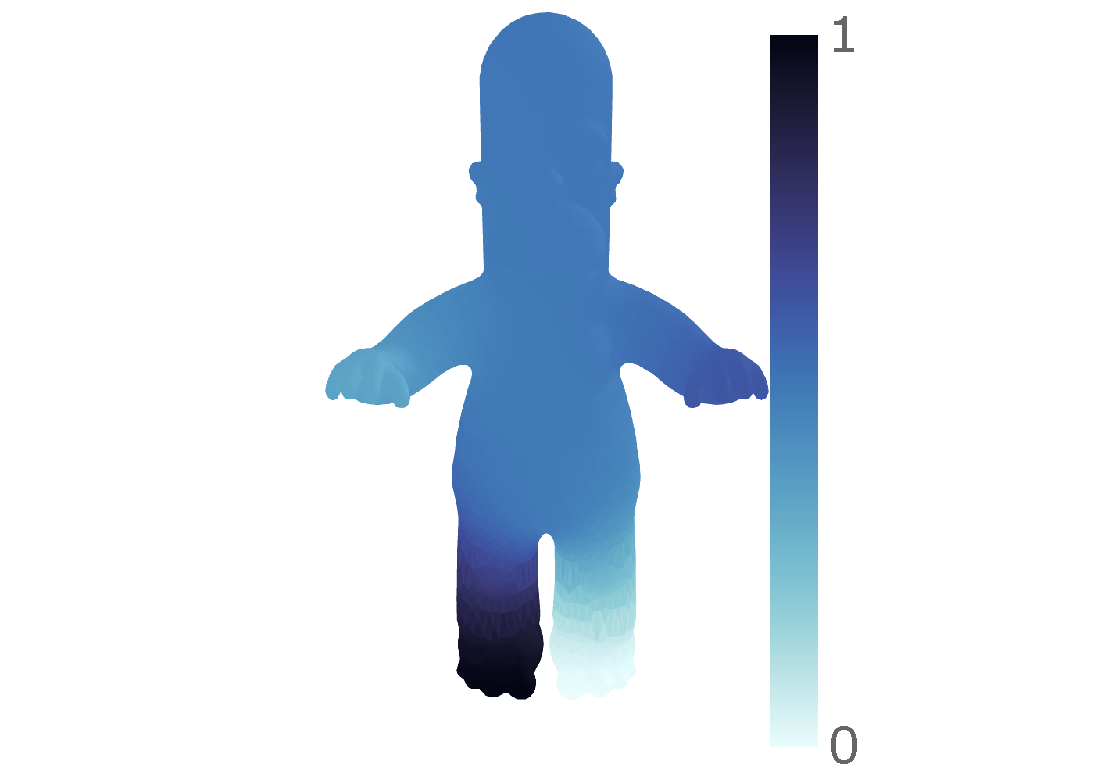
\includegraphics[trim={156 8 21 6},clip,width=.25\textwidth]{homer_rank4_lam2-706937e-03_norm.pdf}} % chktex 8
	\hfill
	\subfloat[\(\mesh{\phi_{6}}\)]
	{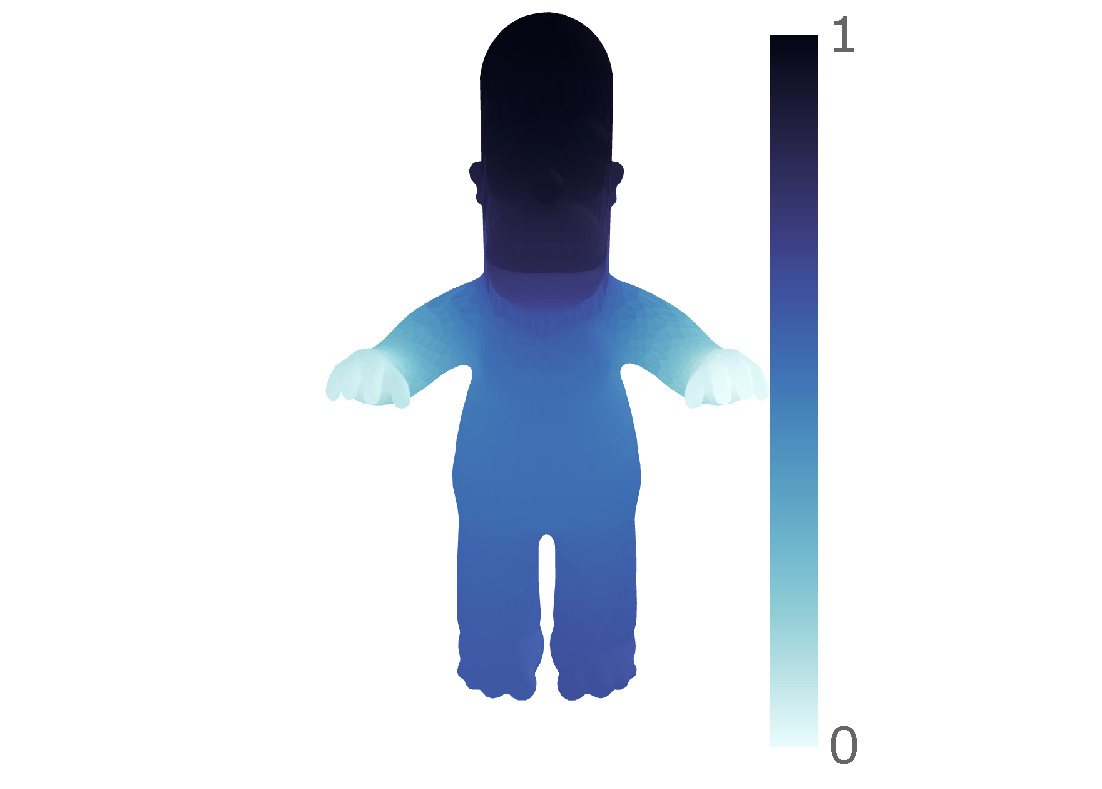
\includegraphics[trim={156 8 21 6},clip,width=.25\textwidth]{homer_rank5_lam2-851096e-03_norm.pdf}} % chktex 8
	\newline
	\subfloat[\(\mesh{\phi_{7}}\)]
	{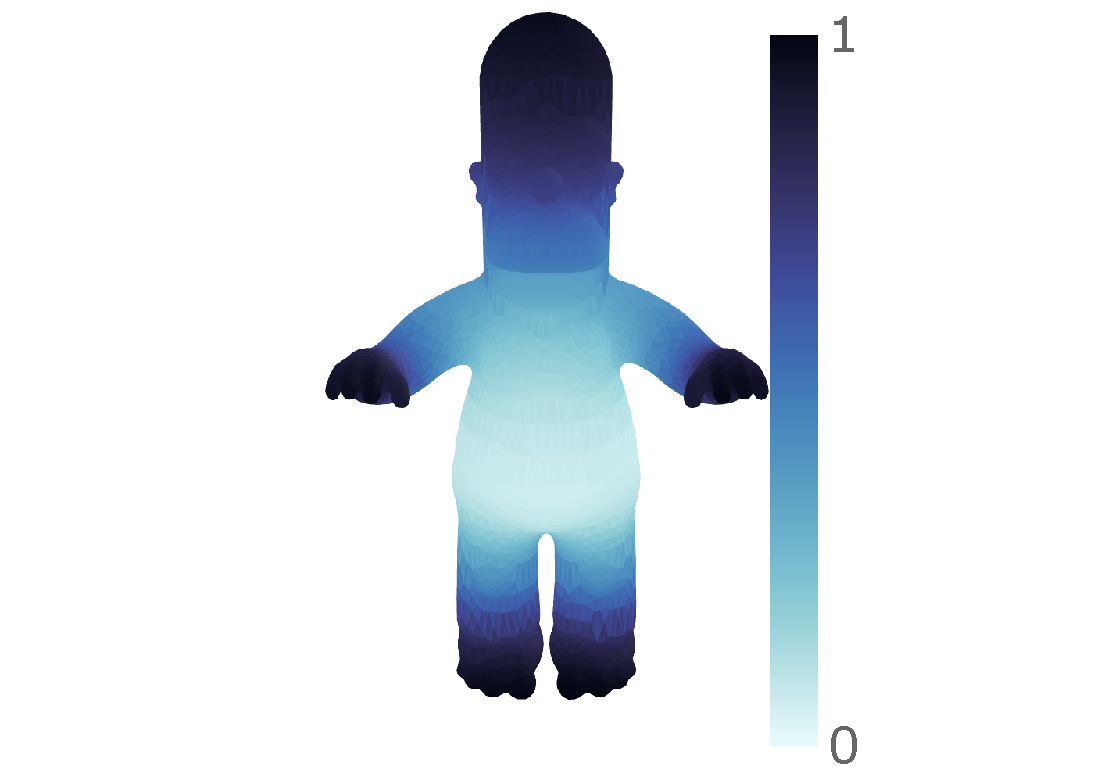
\includegraphics[trim={156 8 21 6},clip,width=.25\textwidth]{homer_rank6_lam7-806422e-03_norm.pdf}} % chktex 8
	\hfill
	\subfloat[\(\mesh{\phi_{8}}\)]
	{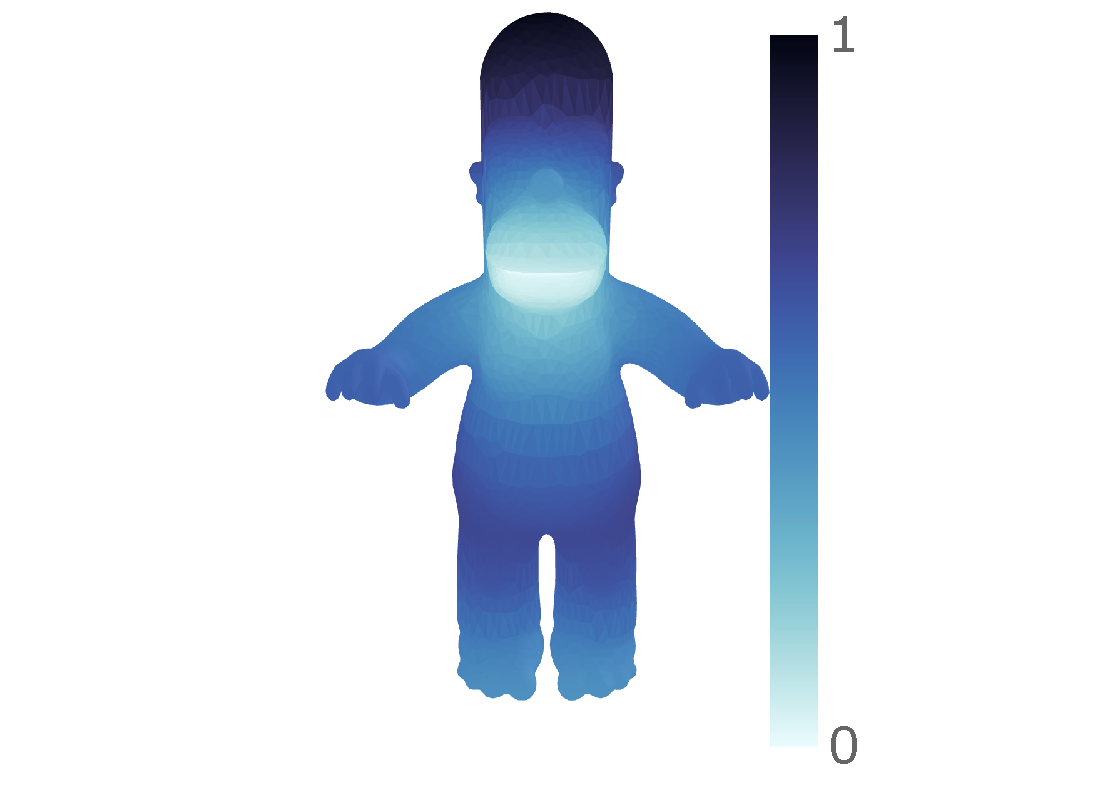
\includegraphics[trim={156 8 21 6},clip,width=.25\textwidth]{homer_rank7_lam1-164387e-02_norm.pdf}} % chktex 8
	\subfloat[\(\mesh{\phi_{9}}\)]
	{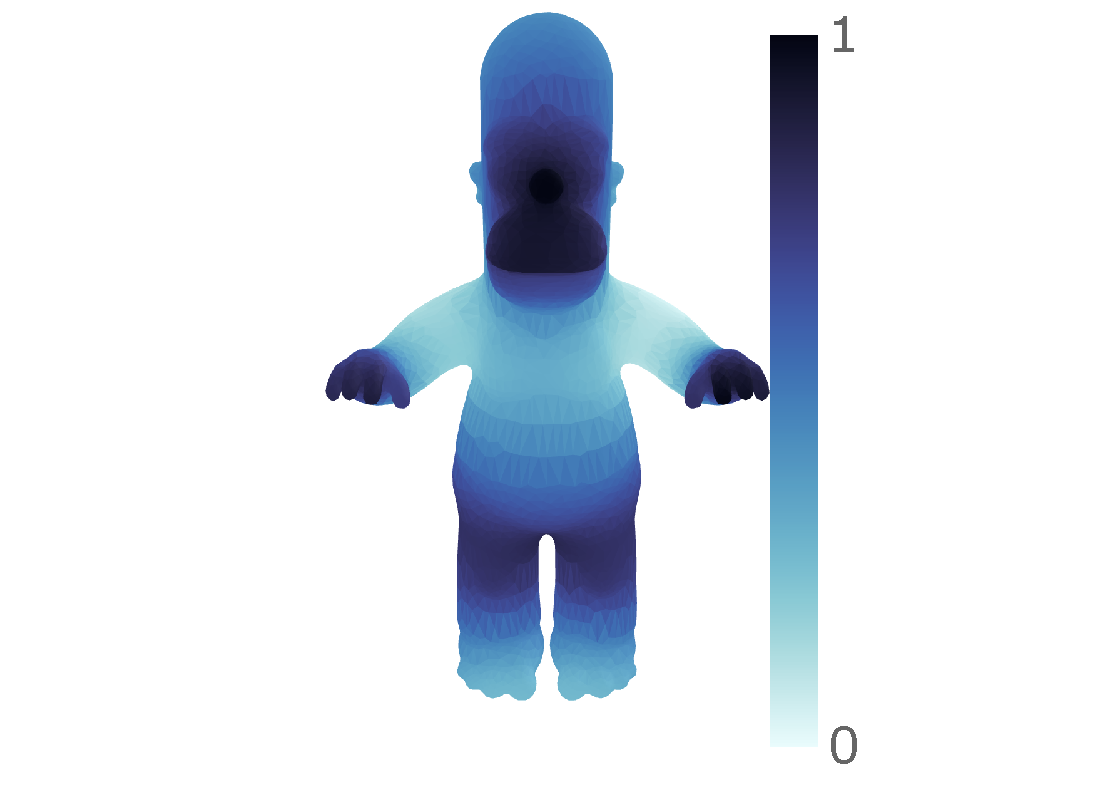
\includegraphics[trim={156 8 21 6},clip,width=.25\textwidth]{homer_rank8_lam1-738974e-02_norm.pdf}} % chktex 8
	\hfill
	\subfloat[\(\mesh{\phi_{10}}\)]
	{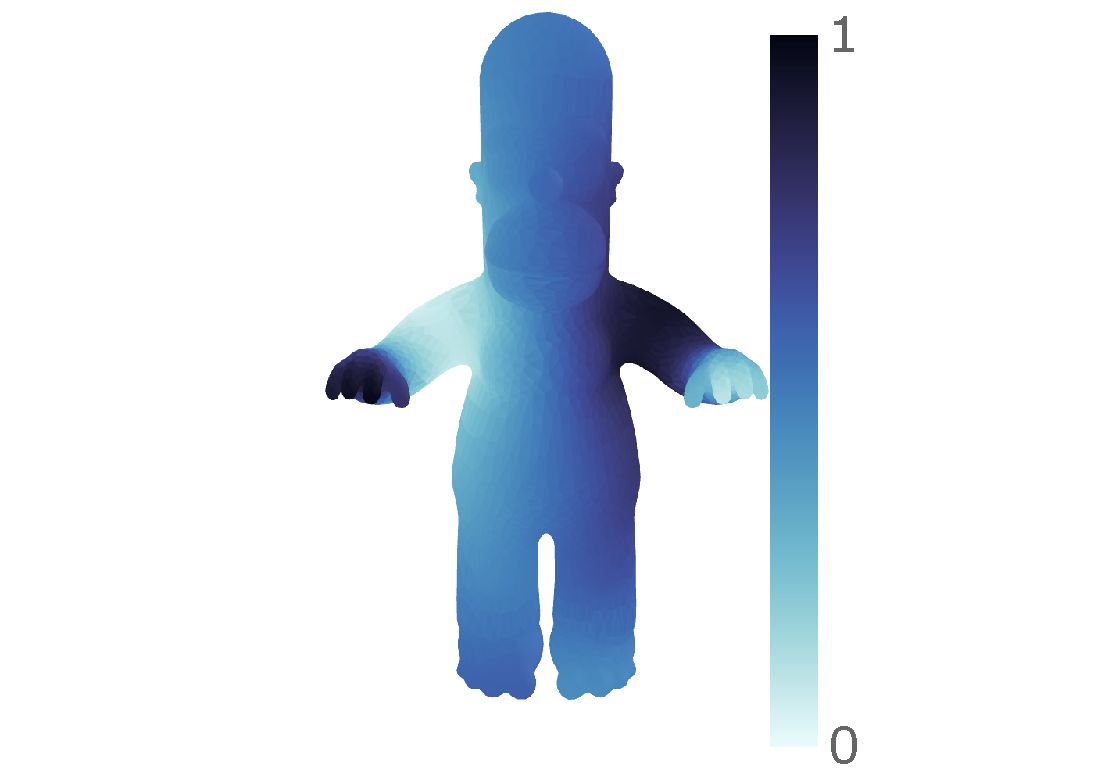
\includegraphics[trim={156 8 21 6},clip,width=.25\textwidth]{homer_rank9_lam1-827015e-02_norm.pdf}} % chktex 8
	\caption{
		The third to tenth eigenvectors of the mesh Laplacian of a Homer Simpson mesh ordered by increasing eigenvalue (frequency).
		In total \(\num{1275}\) basis functions of the \(\num{5103}\) vertex mesh were computed.
		Whilst the eigenvectors are defined on the vertices, the values have been averaged onto the faces for the plot.
	}\label{fig:chapter4_eigenhomers}
\end{figure}


\subsection{Problem Formulation}\label{sec:chapter4_problem_formulation}

This work generalises Slepian scale-discretised wavelets on the sphere~\cite{Roddy2021a} to arbitrary manifolds.
Here, the basis functions of the Slepian concentration problem are built from the eigenfunctions of the Laplace-Beltrami operator/eigenvectors of the graph Laplacian, as opposed to the spherical harmonics.
In the aforesaid work, the wavelets are constructed through a tiling of the Slepian line (akin to the harmonic line) in an analogous manner to~\cite{Wiaux2008,McEwen2018}.
The sifting convolution~\cite{Roddy2021} allows one to perform convolutions where both inputs are directional, whilst the output remains on the sphere.
By leveraging this convolution, the wavelet transforms in the Slepian domain are built on a region of the sphere (\cf{} manifold) to ensure exact reconstruction.
Convolutions are typically not well-defined on manifolds.
The sifting convolution, however, is a product in harmonic space and as such can be applied effectively to manifolds.

In \cref{sec:chapter4_working_with_manifolds}, the Slepian spatial-spectral concentration problem is presented in the manifold setting --- in particular, the spatial concentration of a bandlimited function.
The sifting convolution~\cite{Roddy2021} is then defined similarly, allowing for wavelet transforms on the manifold to be constructed.

\section{Working with Manifolds}\label{sec:chapter4_working_with_manifolds}

In this section a review of the Slepian spatial-spectral concentration problem adapted to manifolds is presented in \cref{sec:chapter4_slepian_concentration_problem_manifolds}.
A review of the sifting convolution follows in \cref{sec:chapter4_sifting_convolution_manifolds} which allows one to perform convolutions on manifolds.

\subsection{Slepian Concentration Problem on Manifolds}\label{sec:chapter4_slepian_concentration_problem_manifolds}

The problem of spatial concentration of bandlimited signals (likewise spectral concentration of spacelimited signals) was first studied by Slepian, Landau and Pollak in the 1960s~\cite{Slepian1961,Landau1961,Landau1962}.
Initially for time domain signals, it has since been extended to other domains such as signals on the sphere~\cite{Simons2006,Roddy2021a,Xu1983,Wieczorek2005}.
This work considers optimally concentrated functions within a region \(R\) of a manifold \(\manifold{}\), an example of which is shown in \cref{fig:chapter4_region}.

% Inspired by Fionn Fitzmaurice's differential geometry notes
% https://gist.github.com/fionn/f27ddeadba97f3dabbf97527b05b33e5
\begin{figure}[htp]
	\centering
	\resizebox{0.75\textwidth}{!}{%
		\begin{tikzpicture}
			\begin{scope}
				\draw [postaction={stipple={amplitude=0.5cm}},
					postaction={stipple={amplitude=0.25cm}}]
				(0, 0) .. controls ++(65:-1.5) and ++(95:1) .. (-1.5, -4)
				(-1.5, -4) .. controls ++(195:-1.3) and ++(195:1) .. (3, -4)
				(3, -4) .. controls ++(95:2) and ++(95:-1) .. (4, 0)
				node[below right] {$\mathcal{M}$}
				(4, 0) .. controls ++(195:1) and ++(195:-1) .. (0, 0);
			\end{scope}
			\draw [use Hobby shortcut, % .. syntax
				closed=true, % connects region outline
				pattern=north east lines] % direction of lines
			(0.7,-2.3) .. (1.2,-2.6) .. (2.3,-2.2) .. (2,-1.8) .. (1.2,-1.3) .. (0.7,-1.4) .. (0.8,-1.9);
			\node at (1.8,-1.3) {\(R\)};
		\end{tikzpicture}%
	}
	\caption{
		In various domains, data are observed on a partial region of a manifold \(\mathcal{M}\), such as \(R\).
	}\label{fig:chapter4_region}
\end{figure}


\subsubsection{Spatial Concentration of a Bandlimited Function}

To maximise the spatial energy concentration of a bandlimited signal \(f \in \hilbert{\manifold}\), the following ratio must be maximised:
%
\begin{equation}
	\mu
	%
	= \frac{\integrateRegion{\meshVolume} \abs{\mesh{f}}^{2}}{\integrateManifold{x} \abs{\mesh{f}}^{2}},
\end{equation}
%
where spatial concentration is measured by \(0 < \mu < 1\).
In harmonic space this can be simplified to a sum
%
\begin{equation}\label{eq:chapter4_spatial_concentration_ratio}
	\mu
	%
	= \frac{\sum\limits_{i} f_{i} \sum\limits_{j} D_{i,j} \conj{f_{j}}}{\meshSum \abs{f_{i}}^{2}},
\end{equation}
%
where
%
\begin{equation}
	D_{i,j}
	%
	= \integrateRegion{\meshVolume \mesh{\phi_{i}} \mesh{\conj{\phi_{j}}}}
\end{equation}
%
is a square matrix including all basis functions of the manifold.
Rewriting \cref{eq:chapter4_spatial_concentration_ratio} as a matrix variational problem
%
\begin{equation}
	\mu
	%
	= \frac{\hermitian{\vb{f}} \vb{D} \vb{f}}{\hermitian{\vb{f}} \vb{f}},
\end{equation}
%
where \(\vb{f}\) are the harmonic coefficients of \(\mesh{f}\), and are the solutions to the eigenproblem
%
\begin{equation}\label{eq:chapter4_eigenproblem}
	\vb{D}\vb{f}
	%
	= \mu \vb{f}.
\end{equation}
%
The eigenvalues \(\mu_{i}\) act as a measure of the relative spatial concentration
%
\begin{equation}
	1 > \mu_{1} \geq \mu_{2} \geq \ldots \geq \mu_{\imax} > 0, % chktex 11
\end{equation}
%
of the corresponding eigenvectors
%
\begin{equation}
	\vb{f}_{1},\ \vb{f}_{2},\ \ldots,\ \vb{f}_{\imax}.
\end{equation}
%
No bandlimited function can be restricted exactly within a region \(R\) and hence \(\mu_{1}<1\).
Due to the positive definiteness of \(\vb{D}\) the smallest eigenvalue \(\mu_{\imax}\) is strictly greater than zero.
A manifold analogue of the \emph{Shannon number} can be constructed by
%
\begin{equation}\label{eq:chapter4_shannon}
	N
	%
	= \frac{A_{R}}{A_{\manifold}} \imax,
\end{equation}
%
where \(A\) denotes the area of the region \(R\)/manifold \(\manifold{}\).
The Shannon number is a good estimate of the number of significant eigenvalues~\cite{Percival1993}.

\subsubsection{Slepian Decomposition}

The Slepian functions provide an alternative orthogonal basis of the manifold, decomposing a function \(f \in \hilbert{\manifold}\) into this basis
%
\begin{equation}
	\mesh{f}
	%
	= \sum\limits_{p=1}^{\imax} \slepian{f} \mesh{\slepian{S}},
\end{equation}
%
where the sum is over all basis functions of the manifold.
For a well-localised function in the region \(R\) (\ie{} \(f \in \hilbert{R}\)) the sum may be truncated at the Shannon number
%
\begin{equation}
	\mesh{f}
	%
	\approx \sum\limits_{p=1}^{N} \slepian{f} \mesh{\slepian{S}}
	%
	= \slepianSum \slepian{f} \mesh{\slepian{S}},
\end{equation}
%
where the last line introduces a shorthand notation.
The Slepian coefficients \(\slepian{f}\) are calculated through the usual projection on to the basis functions
%
\begin{equation}
	\slepian{f}
	%
	= \braket{f}{\slepian{S}}.
\end{equation}

The Slepian coefficients of a well-localised function may be computed with an integral over the region \(R\) rather than an integral over the whole manifold \(\manifold{}\):
%
\begin{equation}
	\slepian{f}
	%
	= \frac{1}{\slepian{\mu}} \integrateRegion{\meshVolume} \mesh{f} \mesh{\conj{\slepian{S}}},
\end{equation}
%
as
%
\begin{align}
	\integrateRegion{\meshVolume} \mesh{f} \mesh{\conj{\slepian{S}}}
	%
	 & = \slepianSum['] \slepian[']{f} \integrateRegion{\meshVolume} \mesh{\slepian[']{S}} \mesh{\conj{\slepian{S}}} \nonumber \\
	%
	 & = \slepianSum['] \slepian[']{f} \hermitian{\slepian{\vb{S}}} \vb{D} \slepian[']{\vb{S}} \nonumber                       \\
	%
	 & = \slepian{f} \slepian{\mu},
\end{align}
%
where \(\vb{S}\) are the harmonic coefficients of \(\mesh{\slepian{S}}\).
Note the use of the orthogonality results
%
\begin{equation}\label{eq:chapter4_orthogonality_manifold}
	\integrateManifold{x} \mesh{\slepian{S}} \mesh{\conj{\slepian[']{S}}}
	%
	= \hermitian{\slepian[']{\vb{S}}} \slepian{\vb{S}}
	%
	= \delta_{pp'},
\end{equation}
%
and
%
\begin{equation}
	\integrateRegion{\meshVolume} \mesh{\slepian{S}} \mesh{\conj{\slepian[']{S}}}
	%
	= \hermitian{\slepian[']{\vb{S}}} \vb{D} \slepian{\vb{S}}
	%
	= \slepian{\mu} \hermitian{\slepian[']{\vb{S}}} \slepian{\vb{S}}
	%
	= \slepian{\mu} \delta_{pp'}.
\end{equation}

To transform from Slepian coefficients to the basis functions of the manifold
%
\begin{equation}\label{eq:chapter4_slepian_to_harmonic}
	f_{i}
	%
	= \integrateManifold{x} \mesh{f} \mesh{\conj{\phi_{i}}}
	%
	= \slepianSum \slepian{f} {(\slepian{S})}_{i},
\end{equation}
%
where \({(\slepian{S})}_{i}\) are the eigenvectors of the eigenproblem \cref{eq:chapter4_eigenproblem}:
%
\begin{equation}
	{(\slepian{S})}_{i}
	%
	= \integrateManifold{x} \mesh{\slepian{S}} \mesh{\conj{\phi_{i}}}.
\end{equation}
%
The inverse operation of \cref{eq:chapter4_slepian_to_harmonic} is
%
\begin{equation}\label{eq:chapter4_harmonic_to_slepian}
	\slepian{f}
	%
	= \integrateManifold{x} \mesh{f} \mesh{\conj{\slepian{S}}}
	%
	= \sum\limits_{i} f_{i} \conj{(\slepian{S})}_{i}.
\end{equation}

\subsection{Sifting Convolution on Manifolds}\label{sec:chapter4_sifting_convolution_manifolds}

A central part of wavelet transforms is the convolution.
On \(\mathbb{R}^{d}\), the convolution of a signal \(f \in \hilbert{\mathbb{R}^{d}}\) with a filter \(g \in \hilbert{\mathbb{R}^{d}}\) is defined by translating \(g\) against \(f\); however, general manifolds do not have well-defined translations.
Recently developed by the authors of this work, the sifting convolution~\cite{Roddy2021} is built on a translation which simply involves a product of the basis functions.
Initially defined in the spherical setting, the sifting convolution can be arbitrarily extended to other domains.

The translation operator on the manifold is
%
\begin{equation}
	\mesh{(\translation{y}\phi_{i})}
	%
	\equiv \meshY{\phi_{i}} \mesh{\phi_{i}},
\end{equation}
%
where \(y\) is a point on the manifold.
An arbitrary function \(f \in \hilbert{\manifold}\) is translated thus
%
\begin{equation}
	\mesh{(\translation{y}f)}
	%
	= \sum\limits_{i} f_{i} \meshY{\phi_{i}} \mesh{\phi_{i}},
\end{equation}
%
implying
%
\begin{equation}
	{(\translation{y}f)}_{i}
	%
	= f_{i} \meshY{\phi_{i}}.
\end{equation}
%
The sifting convolution on the manifold of \(f,\ g \in \hilbert{\manifold}\) follows by the inner product
%
\begin{equation}
	\mesh{\convolution{f}{g}}
	%
	\equiv \integrateManifold{y} \meshY{(\translation{x}f)} \meshY{\conj{g}},
\end{equation}
%
which is a product in harmonic space
%
\begin{equation}
	{\convolution{f}{g}}_{i}
	%
	= f_{i} \conj{g_{i}}.
\end{equation}
%
This convolution can be used to define wavelets restricted to a region of the manifold using the basis functions introduced in \cref{sec:chapter4_slepian_concentration_problem_manifolds} in the translation.

\section{Slepian Wavelets}\label{sec:chapter4_slepian_wavelets}

Here, the Slepian wavelet theory is developed.
Initially, \cref{sec:chapter4_slepian_sifting_convolution} extends the sifting convolution~\cite{Roddy2021} to the Slepian domain.
With a convolution to hand, the Slepian wavelet transform is developed in \cref{sec:chapter4_slepian_scale_discretised_wavelets} --- where an appropriate admissibility condition must hold for exact reconstruction.
The generating functions that define the wavelets are presented in \cref{sec:chapter4_generating_functions}.
Lastly, some properties of the wavelets are discussed in \cref{sec:chapter4_properties}.

\subsection{Slepian Sifting Convolution}\label{sec:chapter4_slepian_sifting_convolution}

To construct wavelets in a region of the manifold a suitable convolution is required.
The sifting convolution on the manifold defined in \cref{sec:chapter4_slepian_concentration_problem_manifolds} and developed by the authors of the current article~\cite{Roddy2021}, can be extended to work with the Slepian functions as a basis.

Consider the sifting convolution of a region on a manifold with the Slepian functions as a localised basis.
The translation is defined as such
%
\begin{equation}
	\mesh{(\translation{y}\slepian{S})}
	%
	\equiv \meshY{\slepian{S}} \mesh{\slepian{S}},
\end{equation}
%
where \(y\) is a point on the manifold and \(\mesh{\slepian{S}}\) are the Slepian functions defined in \cref{sec:chapter4_slepian_concentration_problem_manifolds}.
Hence, the translation of an arbitrary function \(f \in \hilbert{R}\) is
%
\begin{equation}
	\mesh{(\translation{y}f)}
	%
	= \slepianSum \slepian{f} \meshY{\slepian{S}} \mesh{\slepian{S}},
\end{equation}
%
which is the following in Slepian space
%
\begin{equation}
	\slepian{(\translation{y}f)}
	%
	= \slepian{f} \mesh{\slepian{S}}.
\end{equation}
%
As before, the sifting convolution between two functions \(f,\ g \in \hilbert{R}\) is
%
\begin{equation}
	\mesh{\convolution{f}{g}}
	%
	\equiv \integrateManifold{y} \meshY{(\translation{x}f)} \meshY{\conj{g}},
\end{equation}
%
which becomes a product in Slepian space
%
\begin{equation}
	\slepian{\convolution{f}{g}}
	%
	= \slepian{f} \conj{\slepian{g}},
\end{equation}
%
and hence is efficient to compute.
Slepian wavelets may now be defined utilising this convolution in Slepian space.

\subsection{Slepian Scale-Discretised Wavelets}\label{sec:chapter4_slepian_scale_discretised_wavelets}

A Slepian wavelet transform can be constructed through a tiling of Slepian space, where \(p\) is restricted to \(N=\imax A_{R}/A_{\manifold}\) (or \(\imax{}\) for whole manifold).
Spatially localised, scale-dependent content of a signal may be probed through a scale-discretised wavelet transform.
The construction of these wavelets is in an analogous manner to~\cite{Wiaux2008,McEwen2018} but are computed in the Slepian basis rather than the basis functions of the sphere (\cf{} manifold).

For a signal of interest \(f \in \hilbert{R}\) concentrated within a region \(R\), the wavelet coefficients \(W^{\Psi^{j}} \in \hilbert{R}\) are defined through a sifting convolution of \(f\) with the wavelet \(\Psi^{j} \in \hilbert{R}\) for wavelet scale \(j\):
%
\begin{align}
	\mesh{W^{\Psi^{j}}}
	%
	 & = \mesh{\convolution{\Psi^{j}}{f}} \nonumber                                \\
	%
	 & = \integrateManifold{y} \meshY{(\translation{x}\Psi^{j})} \meshY{\conj{f}}.
\end{align}
%
In Slepian space this becomes
%
\begin{equation}\label{eq:chapter4_slepian_wavelet_p}
	\slepian{W}^{\Psi^{j}}
	%
	= \slepian{\Psi}^{j} \conj{\slepian{f}},
\end{equation}
%
where \(\slepian{\Psi}^{j}\) are the Slepian harmonic coefficients of the wavelet at scale \(j\).

Wavelets are typically paired with a scaling function, each capturing different underlying scales of the signal.
Scaling coefficients \(W^{\Phi} \in \hilbert{R}\) may be similarly defined by a sifting convolution between \(f\) and the scaling function \(\Phi \in \hilbert{R}\):
%
\begin{align}
	\mesh{W^{\Phi}}
	%
	 & = \mesh{\convolution{\Phi}{f}} \nonumber                                \\
	%
	 & = \integrateManifold{y} \meshY{(\translation{x}\Phi)} \meshY{\conj{f}},
\end{align}
%
or in Slepian space
%
\begin{equation}\label{eq:chapter4_slepian_scaling_p}
	\slepian{W}^{\Phi}
	%
	= \slepian{\Phi} \conj{\slepian{f}},
\end{equation}
%
where \(\slepian{\Phi}\) are the Slepian coefficients of the scaling function.

Supposing that the wavelets and scaling function satisfy an admissibility condition, a function \(f\) may be reconstructed from its wavelet and scaling coefficients by
%
\begin{equation}\label{eq:chapter4_synthesis}
	\mesh{f}
	%
	= \integrateManifold{y}
	%
	\meshY{(\translation{x}\Phi)} \meshY{W^{\Phi\ast}}
	%
	+ \waveletSum \meshY{(\translation{x}\Psi^{j})} \meshY{W^{\Psi^{j}\ast}},
\end{equation}
%
or in Slepian space
%
\begin{equation}
	\slepian{f}
	%
	= \slepian{W}^{\Phi\ast} \slepian{\Phi}
	%
	+ \waveletSum \slepian{W}^{\Psi^{j}\ast} \slepian{\Psi}^{j}.
\end{equation}
%
The parameters \(J_{0}\) and \(J\) represent the lowest and highest scales \(j\) of the wavelet decomposition respectively --- to ensure exact reconstruction these parameters must be set consistently.
The admissibility condition required for synthesis \cref{eq:chapter4_synthesis} to hold is thus
%
\begin{equation}\label{eq:chapter4_admissibility}
	\abs{\slepian{\Phi}}^{2}
	%
	+ \waveletSum \abs{\slepian{\Psi}^{j}}^{2}
	%
	= 1,\ \forall p.
\end{equation}
%
Wavelets and a scaling function that satisfy this admissibility condition may now be defined.

\subsection{Generating Functions}\label{sec:chapter4_generating_functions}

A tiling of the Slepian line defines the wavelets through smooth generating functions --- in an analogous manner to \cref{sec:chapter3_generating_functions}.
A smoothly decreasing function \(k_{\lambda}\), defined in~\cite{Wiaux2008}, is unity for \(t < 1/\lambda{}\), zero for \(t > 1\), and smoothly decreasing otherwise.
The wavelet generating function is defined as
%
\begin{equation}
	\kappa_{\lambda}(t)
	%
	\equiv \sqrt{k_{\lambda}(t/\lambda) - k_{\lambda}(t)},
\end{equation}
%
and the scaling function generating function is
%
\begin{equation}
	\eta_{\lambda}(t)
	%
	\equiv \sqrt{k_{\lambda}(t)}.
\end{equation}

An instinctive approach is to define the wavelets \(\slepian{\Psi}^{j}\) from the generating functions \(\kappa_{\lambda}\) to have support on \(\interval{\lambda^{j-1}}{\lambda^{j+1}}\), yielding
%
\begin{equation}
	\slepian{\Psi}^{j}
	%
	\equiv \kappa_{\lambda}\bigg(\frac{p}{\lambda^{j}}\bigg).
\end{equation}
%
For \(p \geq \lambda^{J_{0}}\) the admissibility condition \cref{eq:chapter4_admissibility} is satisfied for these wavelets, where \(J_{0}\) is the lowest wavelet scale used in the decomposition.
Modes that cannot be probed by wavelets can be extracted through the construction of a scaling function \(\Phi{}\) (\ie{} modes with \(p < \lambda^{J_{0}}\)):
%
\begin{equation}
	\slepian{\Phi}
	%
	\equiv \eta_{\lambda}\bigg(\frac{p}{\lambda^{J_{0}}}\bigg).
\end{equation}
%
Exact reconstruction can be achieved by setting \(J\) appropriately
%
\begin{equation}
	J = \lceil{} \log_{\lambda}(N)\rceil{}.
\end{equation}
%
Assuming that \(0 \leq J_{0} < J\) is satisfied, the lowest wavelet scale \(J_{0}\) is arbitrary.
The Slepian wavelets are constructed by the tiling of the Slepian line as shown in \cref{fig:chapter4_tiling}.

\begin{figure}[htp]
	\centering
	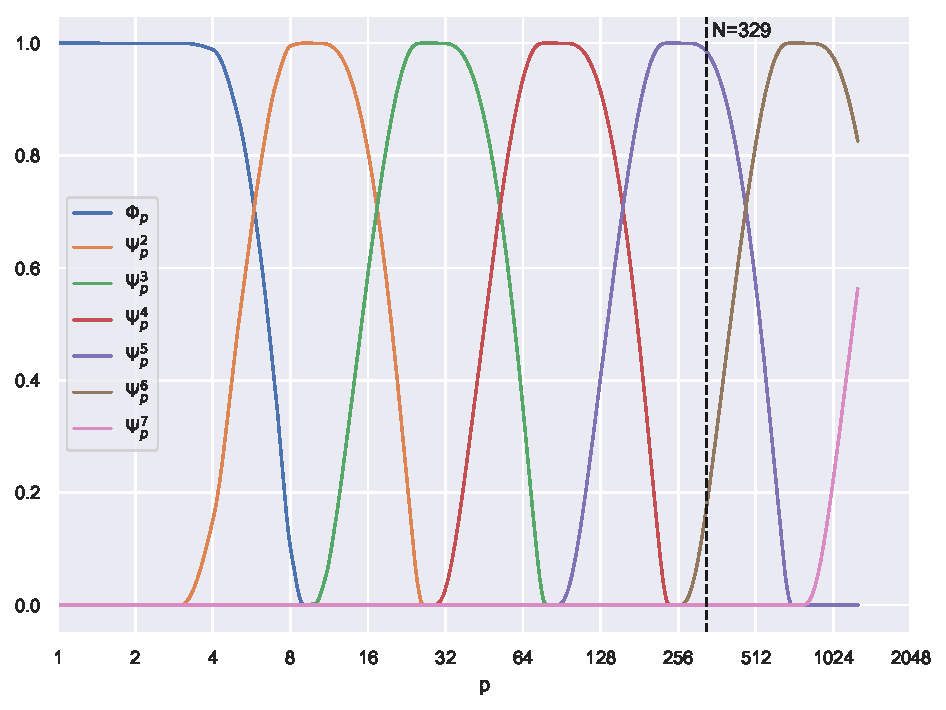
\includegraphics[width=\textwidth]{homer_slepian_tiling_b1275.pdf}
	\caption{
	}\label{fig:chapter4_tiling}
\end{figure}


\subsection{Properties}\label{sec:chapter4_properties}

The properties of Slepian wavelets on manifolds are reviewed here.
In comparison to standard scale-discretised wavelets, the properties are often similar, but not always.

\subsubsection{Localisation}\label{sec:chapter4_localisation}

A tiling of the harmonic line leads to the usual construction of scale-discretised wavelets.
Hence, the value of \(j\) in the wavelets \(\Psi^{j}\) corresponds to increasingly smaller scales (higher frequencies).
However, in the Slepian setting \(p\) is a measure of spatial concentration, where a lower \(p\) corresponds to better localisation of the Slepian function.
As Slepian wavelets are built on a tiling of the Slepian harmonic line, the localisation is captured in the wavelets and wavelet coefficients.

\subsubsection{Wavelet Energy}

The wavelet energy is
%
\begin{equation}
	\norm{\Psi^{j}}^{2}
	%
	= \integrateManifold{x} \abs{\mesh{\Psi^{j}}}^{2}
	%
	= \slepianSum \abs{\slepian{\Psi}^{j}}^{2}.
\end{equation}
%
Similarly, the scaling function energy is
%
\begin{equation}
	\norm{\Phi}^{2}
	%
	= \slepianSum \abs{\slepian{\Phi}}^{2}.
\end{equation}

\subsubsection{Parseval Frame}

A \emph{Parseval frame} is satisfied by Slepian scale-discretised wavelets on manifolds
%
\begin{equation}
	A\norm{f}^{2} \leq \integrateManifold{x}
	%
	\abs{\braket{\translation{x}\Phi}{f}}^{2}
	%
	+ \waveletSum \abs{\braket{\translation{x}\Psi^{j}}{f}}^{2}
	%
	\leq B\norm{f}^{2},
\end{equation}
%
where \(A,\ B \in \realPosParam{}\).
Proving this requires the definition in Slepian space of the scaling coefficients \cref{eq:chapter4_slepian_scaling_p} and the wavelet coefficients \cref{eq:chapter4_slepian_wavelet_p}, along with the orthogonality of the Slepian functions \cref{eq:chapter4_orthogonality_manifold}
%
\begin{equation}
	\slepianSum \abs{\slepian{\Phi}}^{2} \abs{\slepian{f}}^{2}
	%
	+ \waveletSum \abs{\slepian{\Psi}^{j}}^{2} \abs{\slepian{f}}^{2}
	%
	= \norm{f}^{2},
\end{equation}
%
where the admissibility condition \cref{eq:chapter4_admissibility} results in the final equality.
Therefore, a Parseval frame holds for scale-discretised wavelets with \(A = B = 1\), which implies that the energy of \(f\) is conserved in wavelet space.

\subsubsection{Wavelet Domain Variance}

For notational brevity define a quantity
%
\begin{equation}
	\varphi \in \set{\Phi,\Psi^{j}}
\end{equation}
%
to represent both the scaling function and the wavelets.
The variance of the wavelet/scaling coefficients is given by
%
\begin{equation}
	\variance{\mesh{W^{\varphi}}}
	%
	= \expval{\abs{\mesh{W^{\varphi}}}^{2}}
	%
	-\abs{\expval{\mesh{W^{\varphi}}}}^{2},
\end{equation}
%
where the expected value of the wavelet/scaling coefficients is zero for the common case of zero-mean Gaussian noise.
Thus, the variance can be expanded to become
%
\begin{equation}\label{eq:chapter4_slepian_isotropic_noise}
	\variance{\mesh{W^{\varphi}}}
	%
	= \slepianSum \slepianSum['] \slepian{\varphi} \conj{\slepian[']{\varphi}} \mesh{\slepian{S}} \mesh{\conj{\slepian[']{S}}} \expval{\conj{\slepian{f}} \slepian[']{f}}.
\end{equation}

Consider homogenous and isotropic noise defined by its power spectrum
%
\begin{equation}
	\expval{f_{i} \conj{f_{j}}}
	%
	= C_{i} \delta_{i j},
\end{equation}
%
where \(C_{i} = \sigma^{2}\) for white noise.
The power expression in Slepian space can be found by
%
\begin{align}
	\expval{\slepian{f} \conj{\slepian[']{f}}}
	%
	 & = \sum\limits_{i} \sum\limits_{j} \expval{f_{i} \conj{f_{j}}} \empty{} \conj{(\slepian{S})}_{i} {(\slepian[']{S})}_{j} \nonumber \\
	%
	 & = \sigma^{2} \delta_{pp'},
\end{align}
%
where the first line follows from \cref{eq:chapter4_harmonic_to_slepian}, and the last line follows from the orthogonality of the Slepian functions \cref{eq:chapter4_orthogonality_manifold}.
Hence, the final expression for the wavelet domain variance is
%
\begin{equation}
	\variance{\mesh{W^{\varphi}}}
	%
	= \sigma^{2} \slepianSum \abs{\slepian{\varphi}}^{2} \abs{\mesh{\slepian{S}}}^{2},
\end{equation}
%
and as such the variance depends on the position on the manifold.

\section{Numerical Illustration}\label{sec:chapter4_numerical_illustration}

In this section the construction and application of Slepian wavelets for an example region on a mesh (\cf{} manifold) is demonstrated.
The Slepian functions and eigenvalues of a region of a Homer Simpson mesh are presented in \cref{sec:chapter4_homer_region}.
A field is constructed on the region of the mesh in \cref{sec:chapter4_wavelet_transform}, and the resulting wavelets and wavelet coefficients are computed.
A possible use of Slepian wavelets is shown in \cref{sec:chapter4_wavelet_denoising} through a straightforward denoising procedure.
All computations are performed with the \texttt{S2LET}\footnote{\url{http://astro-informatics.github.io/s2let/}}~\cite{Leistedt2013} code, which enables the construction of the wavelet generating functions discussed in \cref{sec:chapter4_generating_functions}.

\subsection{Homer Region}\label{sec:chapter4_homer_region}

A region of a manifold is created on a mesh of Homer Simpson, \cref{fig:chapter4_homer_region} presents the masked region of Homer's head.
The Slepian functions of this region are computed by solving the eigenproblem \cref{eq:chapter4_eigenproblem}, and then performing an inverse harmonic transform.
The resulting Shannon number \cref{eq:chapter4_shannon} of the region \(R\) is \(N=329\).
A set of Slepian functions of the mesh are shown in \cref{fig:chapter4_slepian_functions} for \(p \in \set{1, 10, 25, 50, 100, 200}\).
Comparing panel (f) to panel (a) one can see that the latter Slepian functions are more spread out in the region, representing worse concentration.
The corresponding eigenvalues \(\slepian{\mu}\) are a measure of spatial concentration, which remain \(\almost{1}\) for many \(p\) values before rapidly decreasing towards zero around \(N\).
The first \(N\) eigenvalues of this Homer region are shown in \cref{fig:chapter4_slepian_eigenvalues}, were the plot to extend to all \(\imax{}\) Slepian eigenvalues then the rest of the eigenvalues would be \(\almost{0}\).

\begin{figure}[htp]
	\centering\capstart{}
	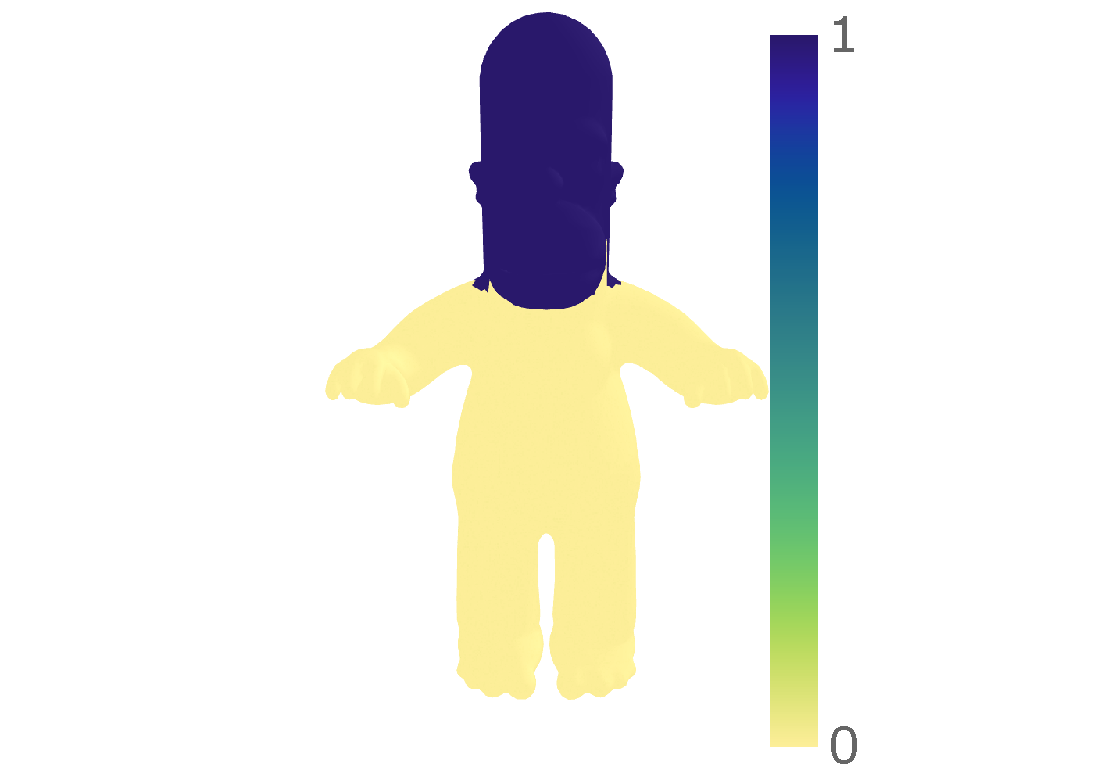
\includegraphics[trim={156 8 21 6},clip,width=.7\textwidth]{homer_region_norm.pdf}
	\caption[
		The head region of the Homer mesh
	]{
		The head region (in blue) chosen to compute the Slepian functions of the Homer mesh.
	}\label{fig:chapter4_homer_region}
\end{figure}


\begin{figure}[htp]
	\centering
	\subfloat[\(\mesh{S_{1}},\ \mu=1.00\)]
	{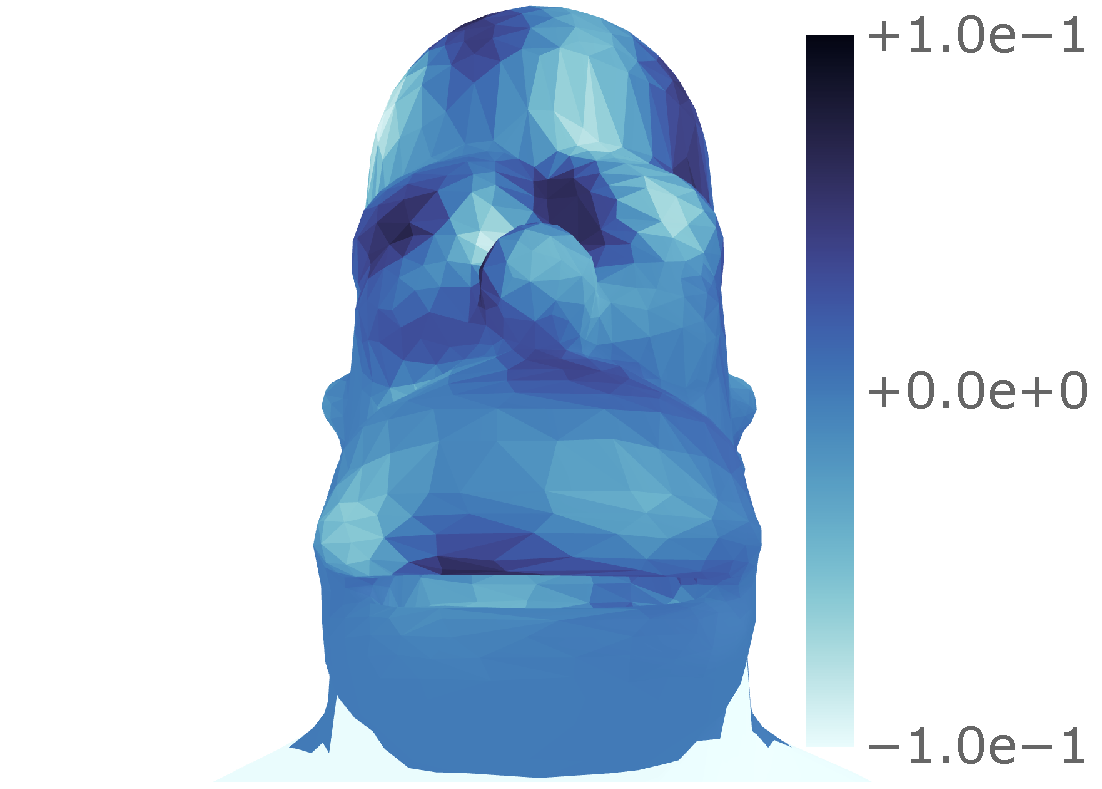
\includegraphics[trim={101 0 3 3},clip,width=.33\textwidth]{slepian_homer_rank0_lam1-000000e00_zoom.pdf}} % chktex 8
	\hfill
	\subfloat[\(\mesh{S_{10}},\ \mu=1.00\)]
	{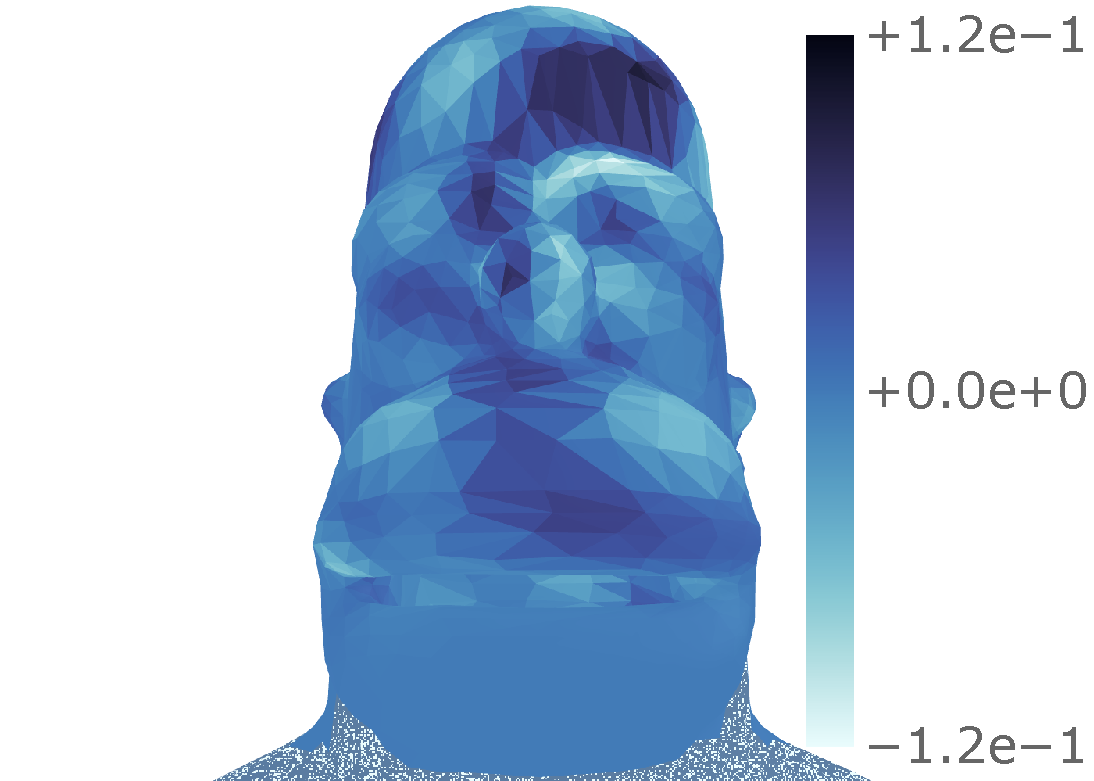
\includegraphics[trim={101 0 3 3},clip,width=.33\textwidth]{slepian_homer_rank9_lam1-000000e00_zoom.pdf}} % chktex 8
	\hfill
	\subfloat[\(\mesh{S_{25}},\ \mu=1.00\)]
	{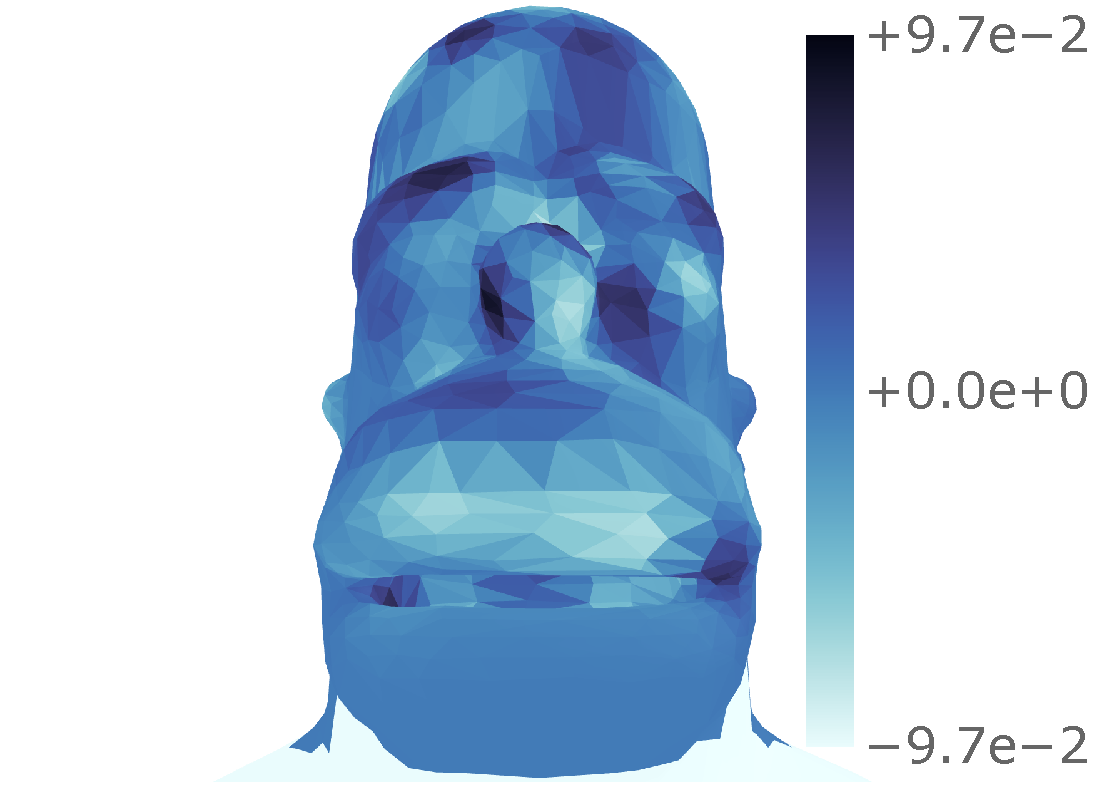
\includegraphics[trim={101 0 3 3},clip,width=.33\textwidth]{slepian_homer_rank24_lam1-000000e00_zoom.pdf}} % chktex 8
	\newline
	\subfloat[\(\mesh{S_{50}},\ \mu=1.00\)]
	{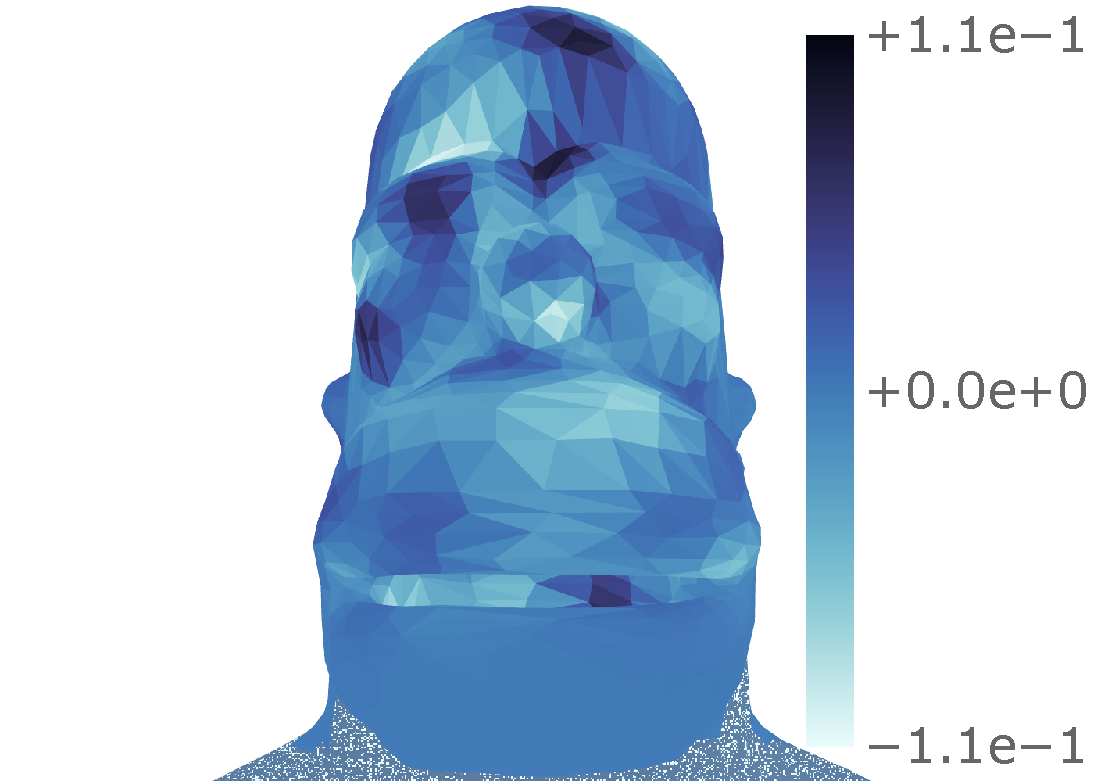
\includegraphics[trim={101 0 3 3},clip,width=.33\textwidth]{slepian_homer_rank49_lam1-000000e00_zoom.pdf}} % chktex 8
	\hfill
	\subfloat[\(\mesh{S_{100}},\ \mu=1.00\)]
	{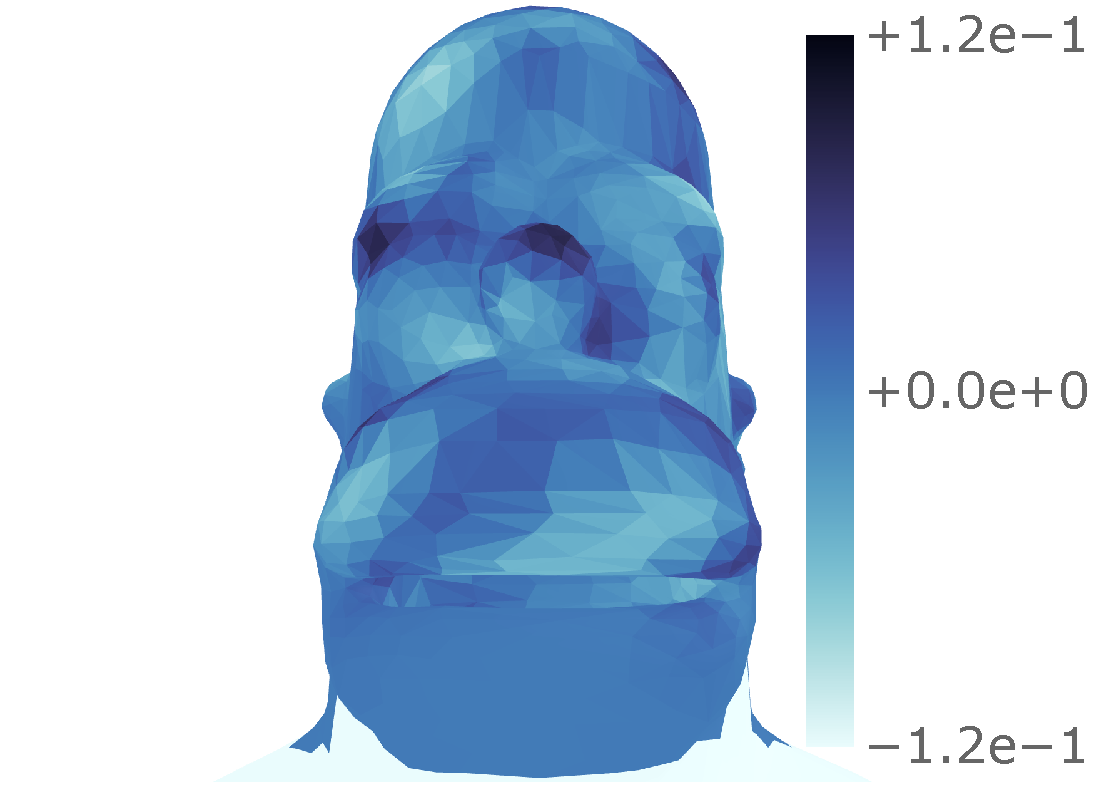
\includegraphics[trim={101 0 3 3},clip,width=.33\textwidth]{slepian_homer_rank99_lam1-000000e00_zoom.pdf}} % chktex 8
	\hfill
	\subfloat[\(\mesh{S_{200}},\ \mu=1.00\)]
	{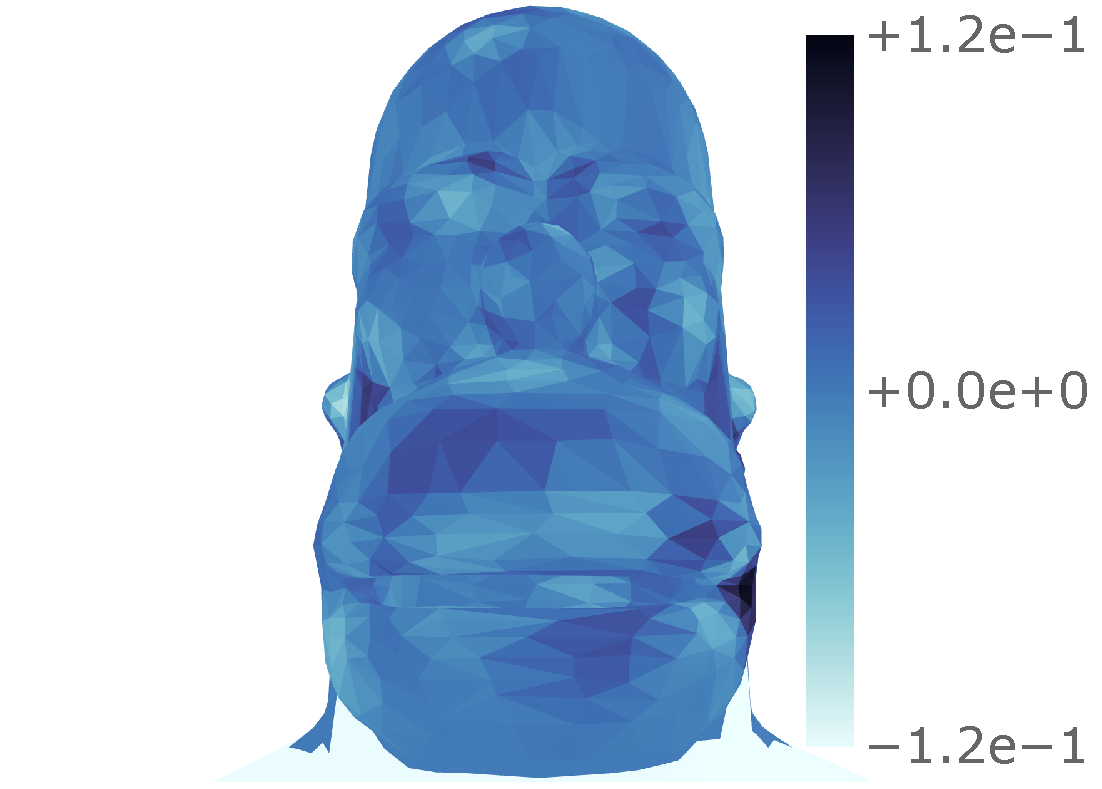
\includegraphics[trim={101 0 3 3},clip,width=.33\textwidth]{slepian_homer_rank199_lam1-000000e00_zoom.pdf}} % chktex 8
	\caption[
		Some Slepian functions of the Homer head region
	]{
		The Slepian functions of the Homer head region \(\mesh{\slepian{S}}\) for \(p \in \set{1, 10, 25, 50, 100, 200}\) shown left-to-right, top-to-bottom.
		The corresponding eigenvalue \(\slepian{\mu}\) is a measure of the concentration within the given region \(R\), which remains \(\almost{1}\) for many \(p\) values before decreasing towards zero.
		Whilst the Slepian functions are defined on the vertices, the values have been averaged onto the faces for the plot.
	}\label{fig:chapter4_slepian_functions}
\end{figure}


\begin{figure}[htp]
	\centering\capstart{}
	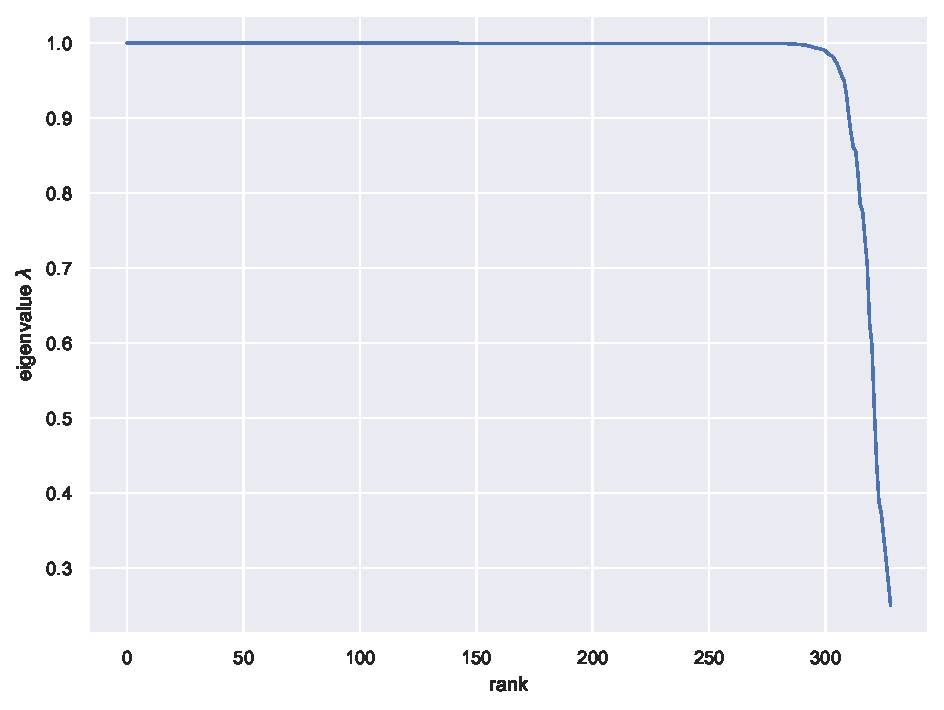
\includegraphics[width=\textwidth]{homer_slepian_eigenvalues_b1275.pdf}
	\caption[
		The Slepian eigenvalues of the Homer head region
	]{
		The eigenvalues of the Homer head region concentrated within the Shannon number \(N=329\).
		The majority of the eigenvalues are \(\almost{1}\) before decreasing rapidly towards zero around the Shannon number.
	}\label{fig:chapter4_slepian_eigenvalues}
\end{figure}


\subsection{Wavelet Transform}\label{sec:chapter4_wavelet_transform}

The Slepian scaling function and wavelets defined in \cref{sec:chapter4_slepian_scale_discretised_wavelets} are built on a tiling of the Slepian line with parameters \(\lambda=3\) and \(J_{0}=2\).
This tiling is shown in \cref{fig:chapter4_tiling} for \(\num{1275}\) basis functions of the Homer mesh, where the Shannon number \(N=329\) is highlighted.
Hence, for this region the scaling function and wavelets for scales \(j \in \set{2, 3, 4, 5, 6}\) are the only non-zero functions.
These wavelets are presented in \cref{fig:chapter4_wavelets}, which show a similar pattern to the Slepian functions where the scaling function is more concentrated in the region than the wavelet scale \(j=6\).
To perform a scale-discretised wavelet transform one requires a signal on the mesh.
\cref{fig:chapter4_homer_data} presents the such a signal, the \(z\)-component of the per vertex normals of the Homer mesh.
With some data to hand, the scaling and wavelet coefficients of the Homer head region are given in \cref{fig:chapter4_wavelet_coefficients}.

\begin{figure}[htp]
	\centering\capstart
	\subfloat[\(\mesh{\Phi}\)]
	{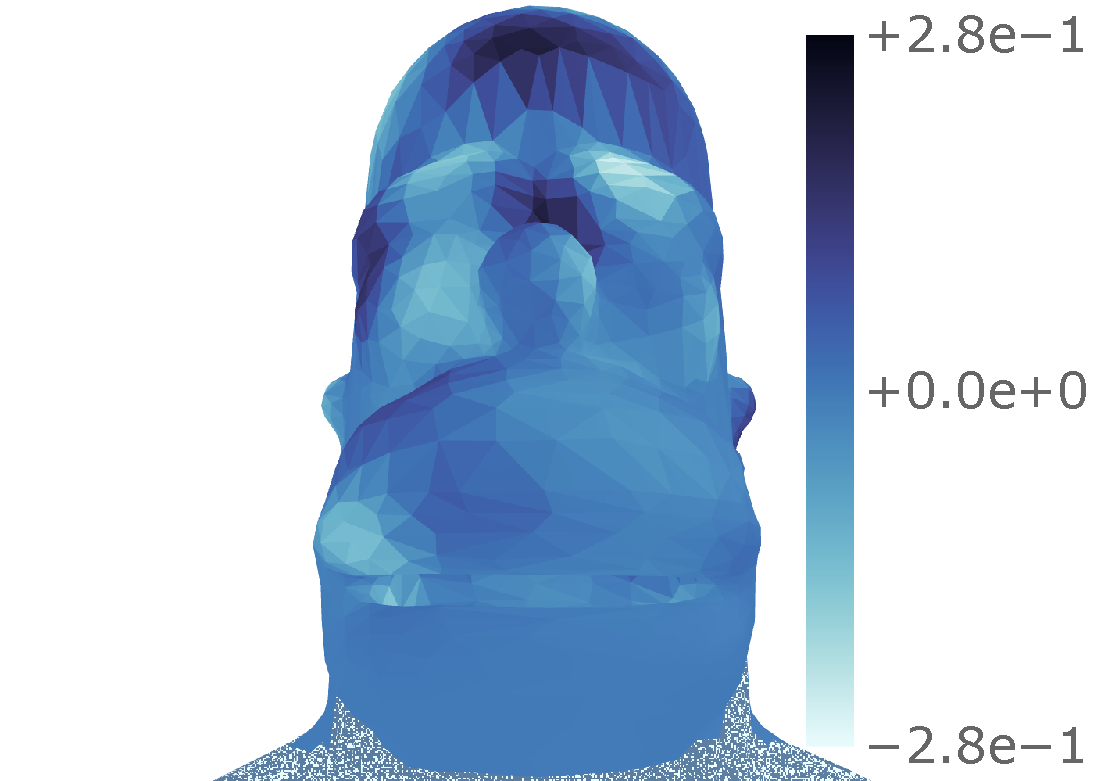
\includegraphics[trim={101 0 3 3},clip,width=.33\textwidth]{slepian_wavelets_homer_3B_2jmin_scaling_zoom.pdf}}
	\hfill
	\subfloat[\(\mesh{\Psi^{2j}}\)]
	{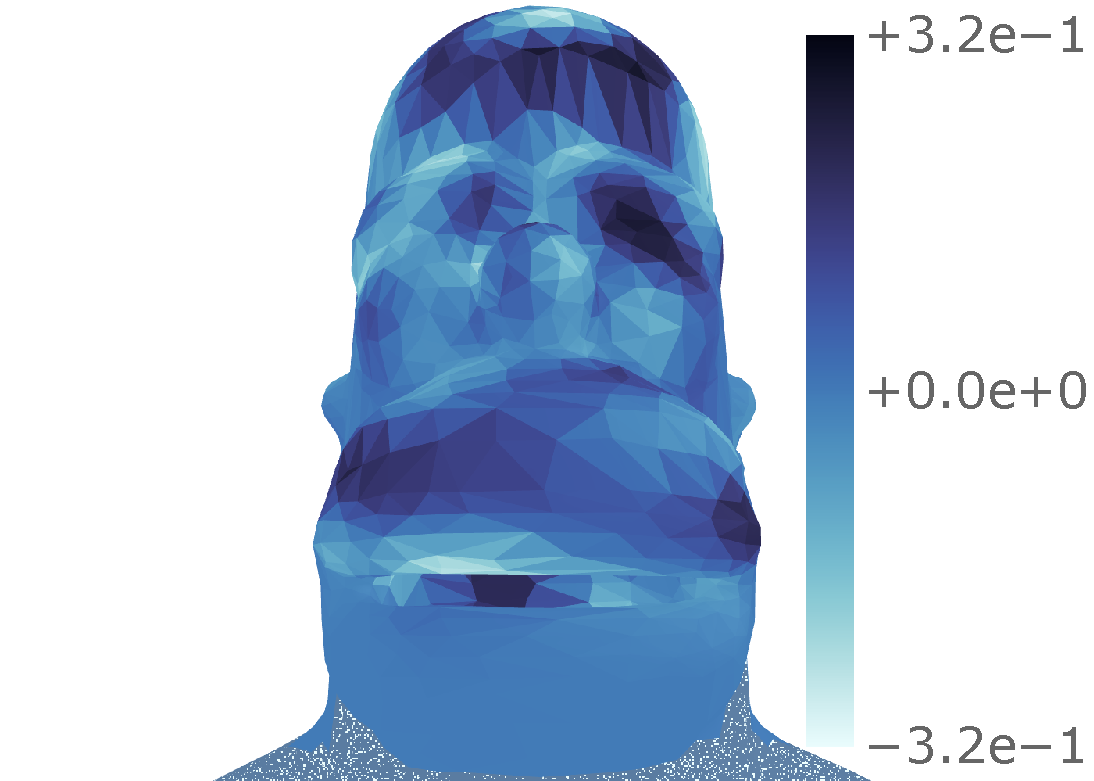
\includegraphics[trim={101 0 3 3},clip,width=.33\textwidth]{slepian_wavelets_homer_3B_2jmin_2j_zoom.pdf}}
	\hfill
	\subfloat[\(\mesh{\Psi^{3j}}\)]
	{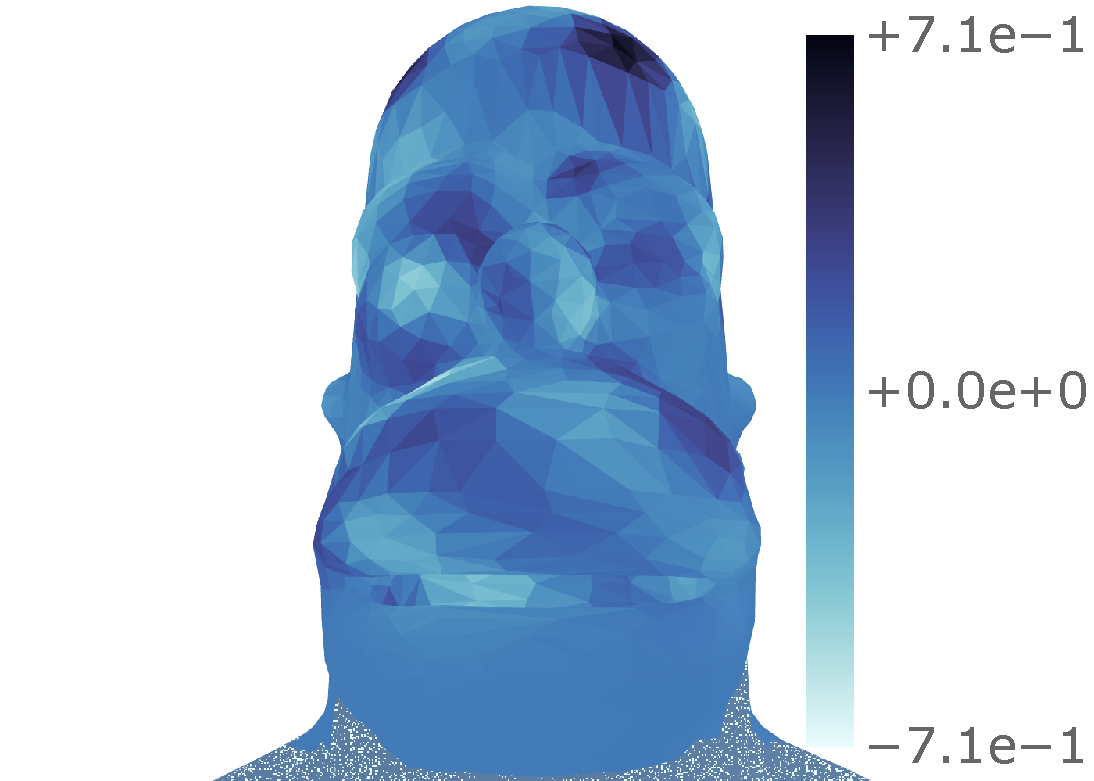
\includegraphics[trim={101 0 3 3},clip,width=.33\textwidth]{slepian_wavelets_homer_3B_2jmin_3j_zoom.pdf}}
	\newline
	\subfloat[\(\mesh{\Psi^{4j}}\)]
	{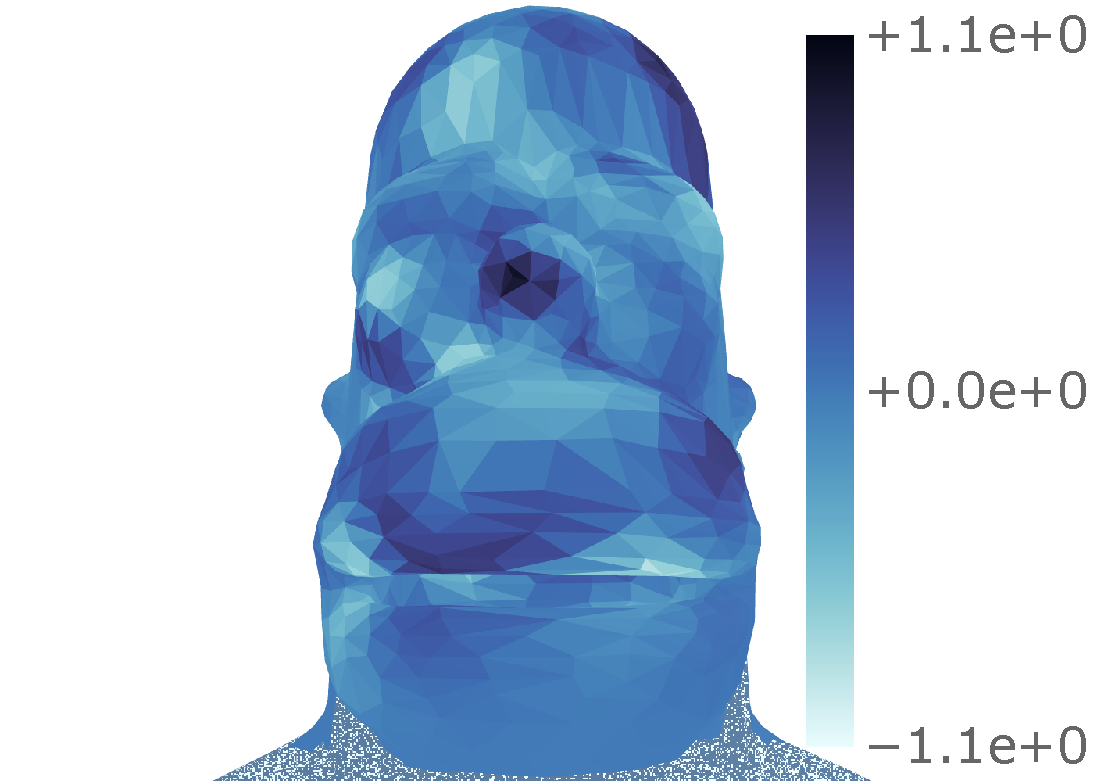
\includegraphics[trim={101 0 3 3},clip,width=.33\textwidth]{slepian_wavelets_homer_3B_2jmin_4j_zoom.pdf}}
	\hfill
	\subfloat[\(\mesh{\Psi^{5j}}\)]
	{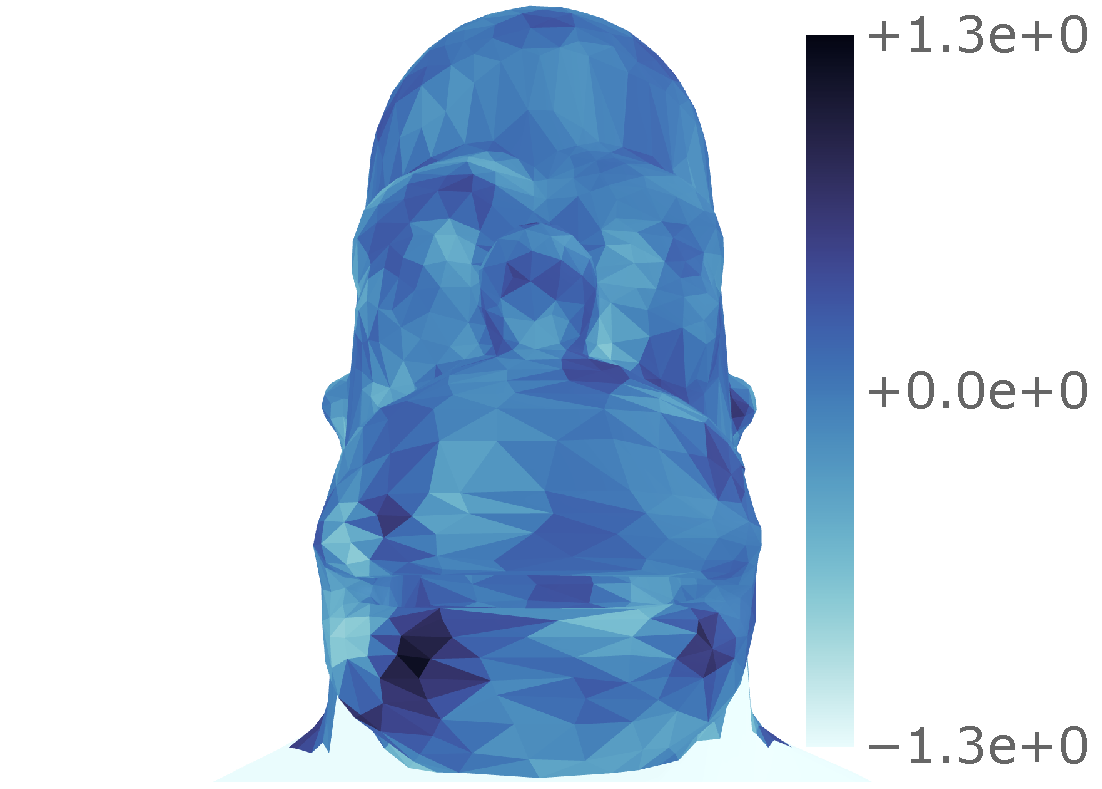
\includegraphics[trim={101 0 3 3},clip,width=.33\textwidth]{slepian_wavelets_homer_3B_2jmin_5j_zoom.pdf}}
	\hfill
	\subfloat[\(\mesh{\Psi^{6j}}\)]
	{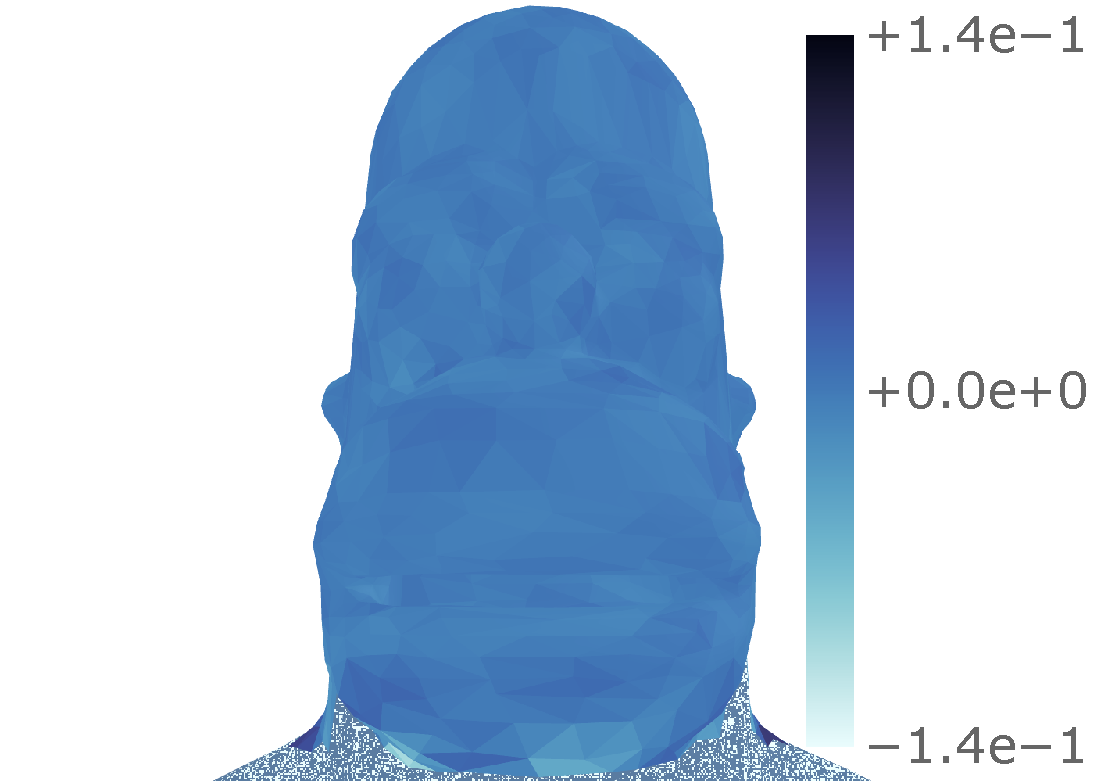
\includegraphics[trim={101 0 3 3},clip,width=.33\textwidth]{slepian_wavelets_homer_3B_2jmin_6j_zoom.pdf}}
	\caption[
		The Slepian wavelets of the Homer head region
	]{
		The scaling function and the wavelets for scales \(j \in \set{2, 3, 4, 5, 6}\) for the Homer head region shown left-to-right, top-to-bottom.
		The wavelets are constructed through a tiling of the Slepian line using scale-discretised functions, with parameters \(\lambda=3\), \(J_{0}=2\), and \(\imax=\num{1275}\) basis functions.
		Whilst the wavelets are defined on the vertices, the values have been averaged onto the faces for the plot.
	}\label{fig:chapter4_wavelets}
\end{figure}


\begin{figure}[htpb]
	\centering\capstart{}
	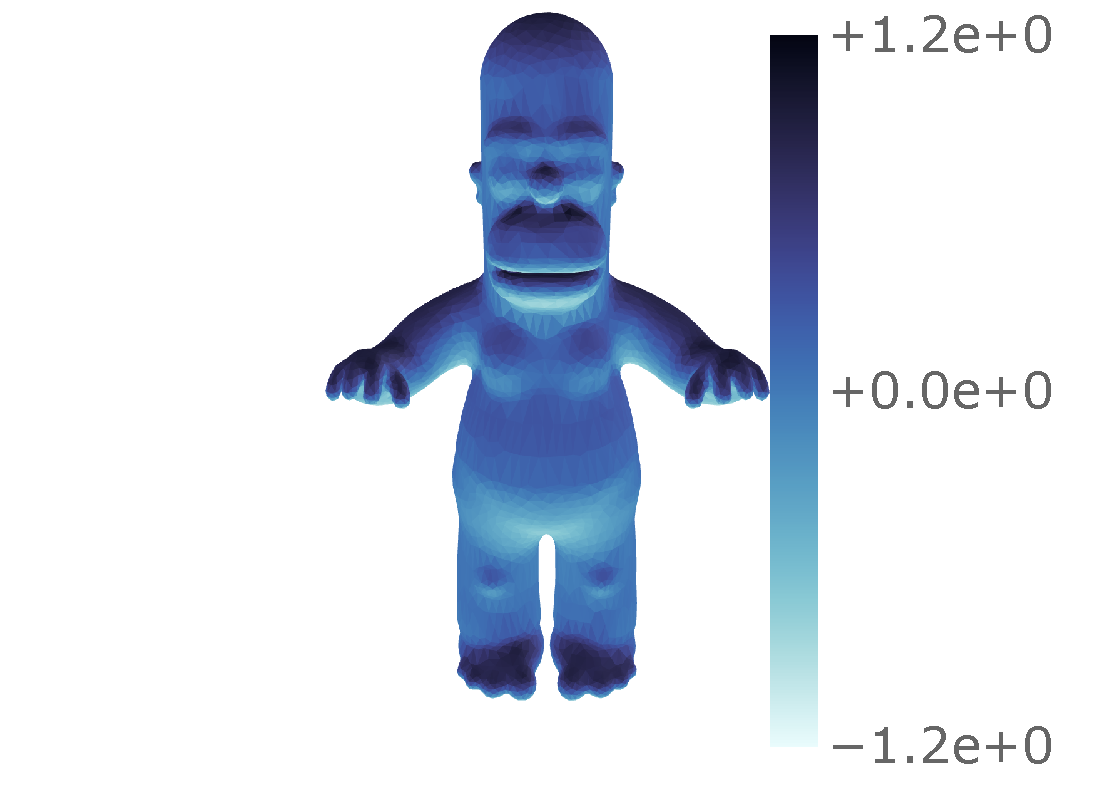
\includegraphics[trim={156 8 21 6},clip,width=.7\textwidth]{homer_field.pdf}
	\caption[
		An example field on the Homer mesh
	]{
		The \(z\)-component of the per vertex normals of the Homer mesh.
		Whilst the field is defined on the vertices, the values have been averaged onto the faces for the plot.
	}\label{fig:chapter4_homer_data}
\end{figure}


\begin{figure}[htp]
	\centering
	\subfloat[\(\mesh{W^{\Phi}}\)]
	{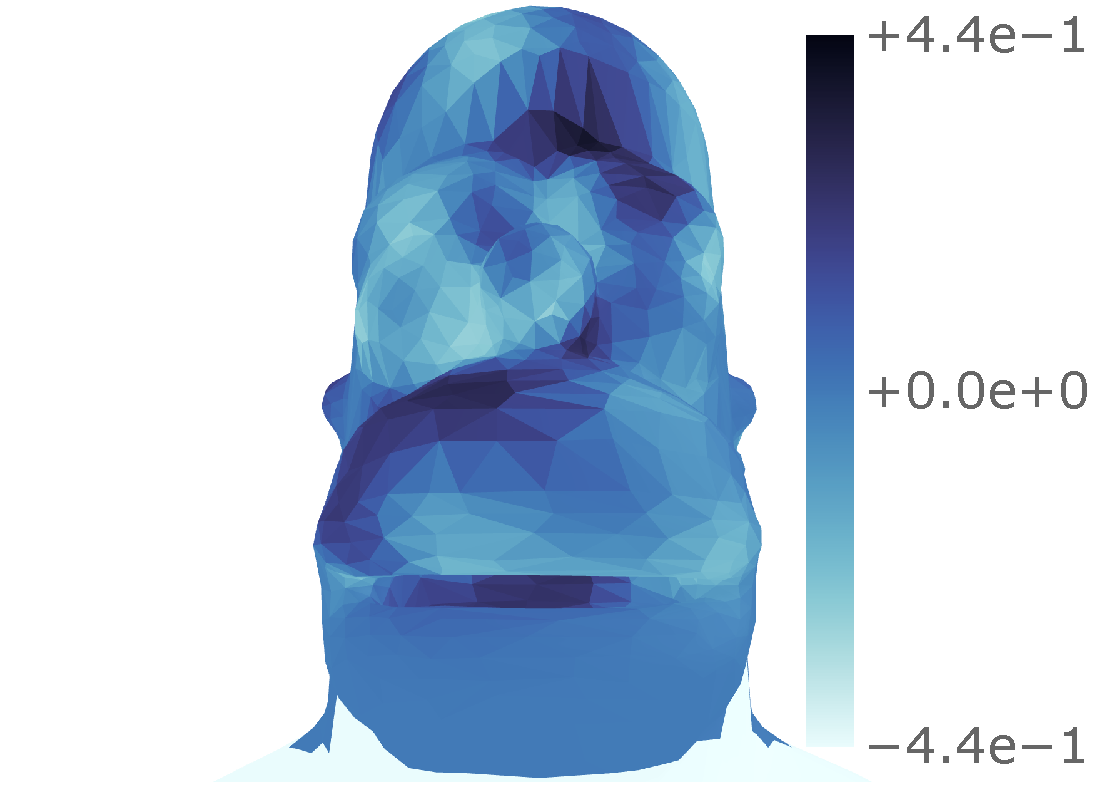
\includegraphics[trim={101 0 3 3},clip,width=.33\textwidth]{slepian_wavelet_coefficients_homer_3B_2jmin_scaling_zoom.pdf}}
	\hfill
	\subfloat[\(\mesh{W^{\Psi^{2j}}}\)]
	{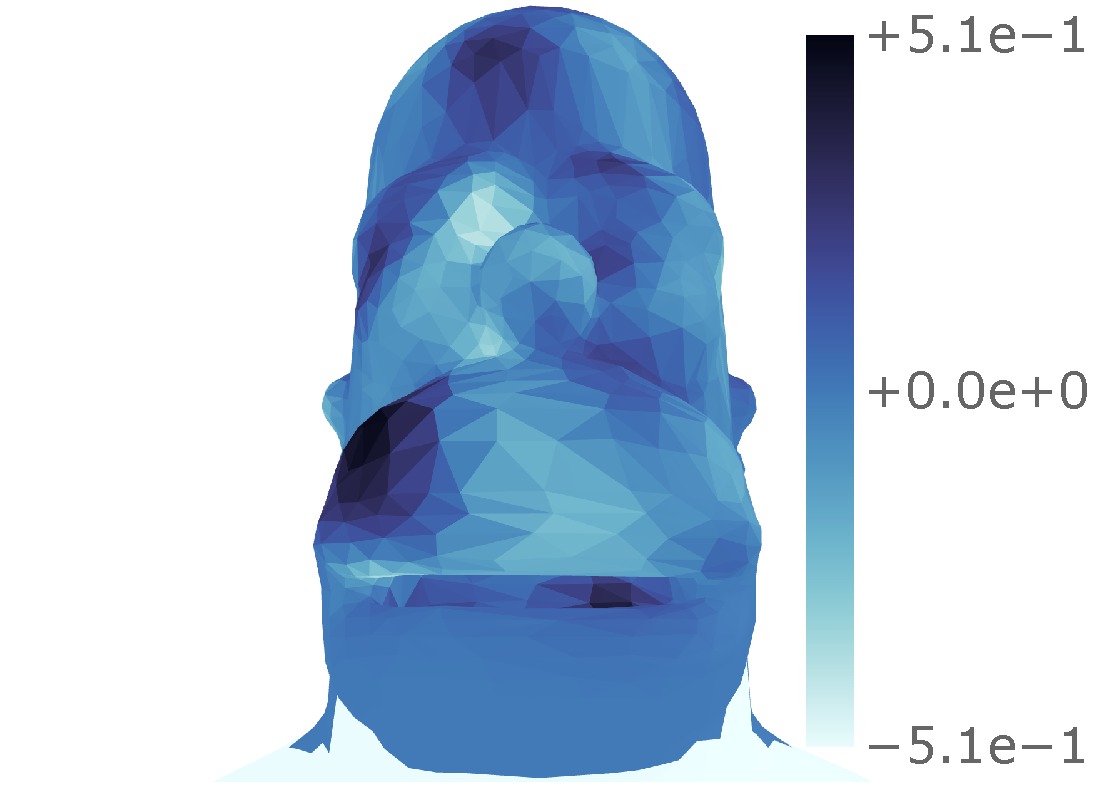
\includegraphics[trim={101 0 3 3},clip,width=.33\textwidth]{slepian_wavelet_coefficients_homer_3B_2jmin_2j_zoom.pdf}}
	\hfill
	\subfloat[\(\mesh{W^{\Psi^{3j}}}\)]
	{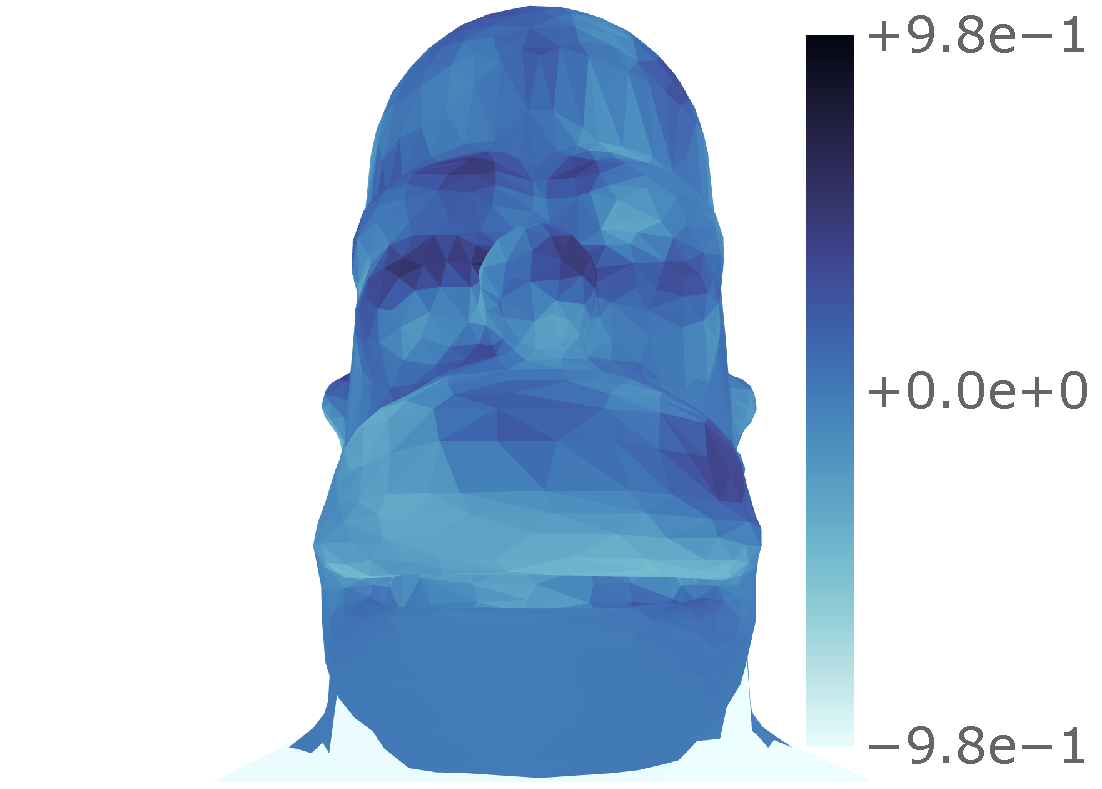
\includegraphics[trim={101 0 3 3},clip,width=.33\textwidth]{slepian_wavelet_coefficients_homer_3B_2jmin_3j_zoom.pdf}}
	\newline
	\subfloat[\(\mesh{W^{\Psi^{4j}}}\)]
	{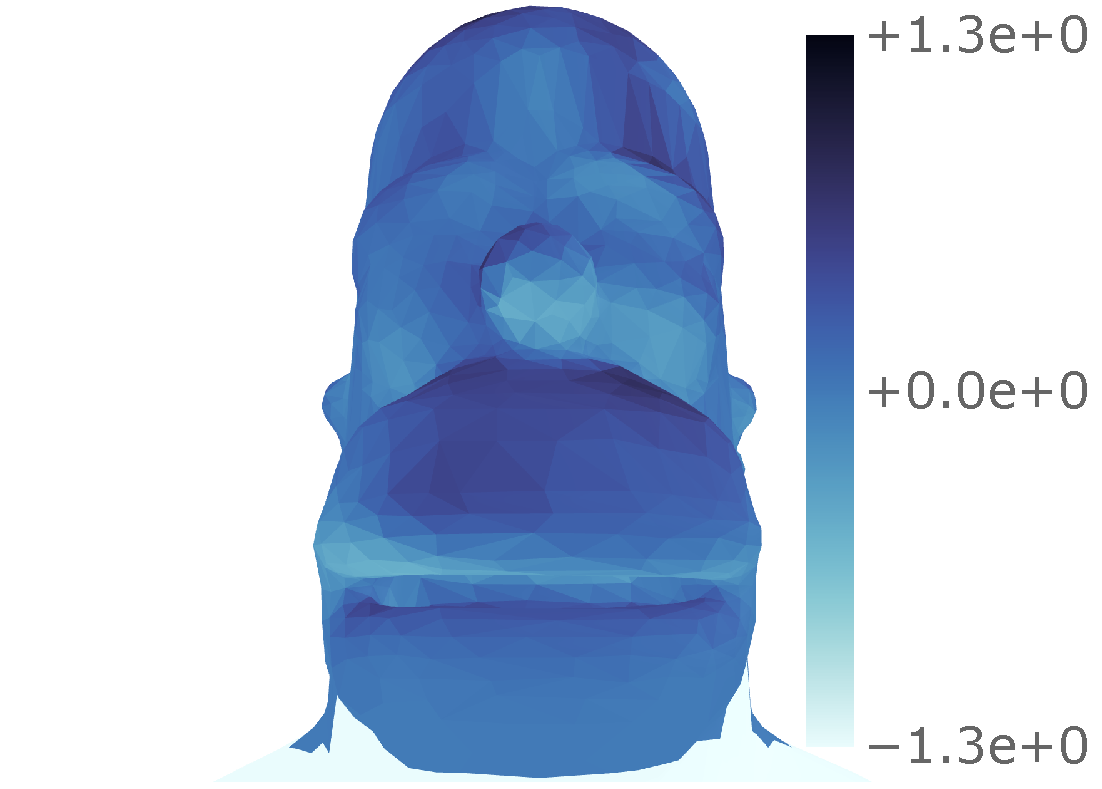
\includegraphics[trim={101 0 3 3},clip,width=.33\textwidth]{slepian_wavelet_coefficients_homer_3B_2jmin_4j_zoom.pdf}}
	\hfill
	\subfloat[\(\mesh{W^{\Psi^{5j}}}\)]
	{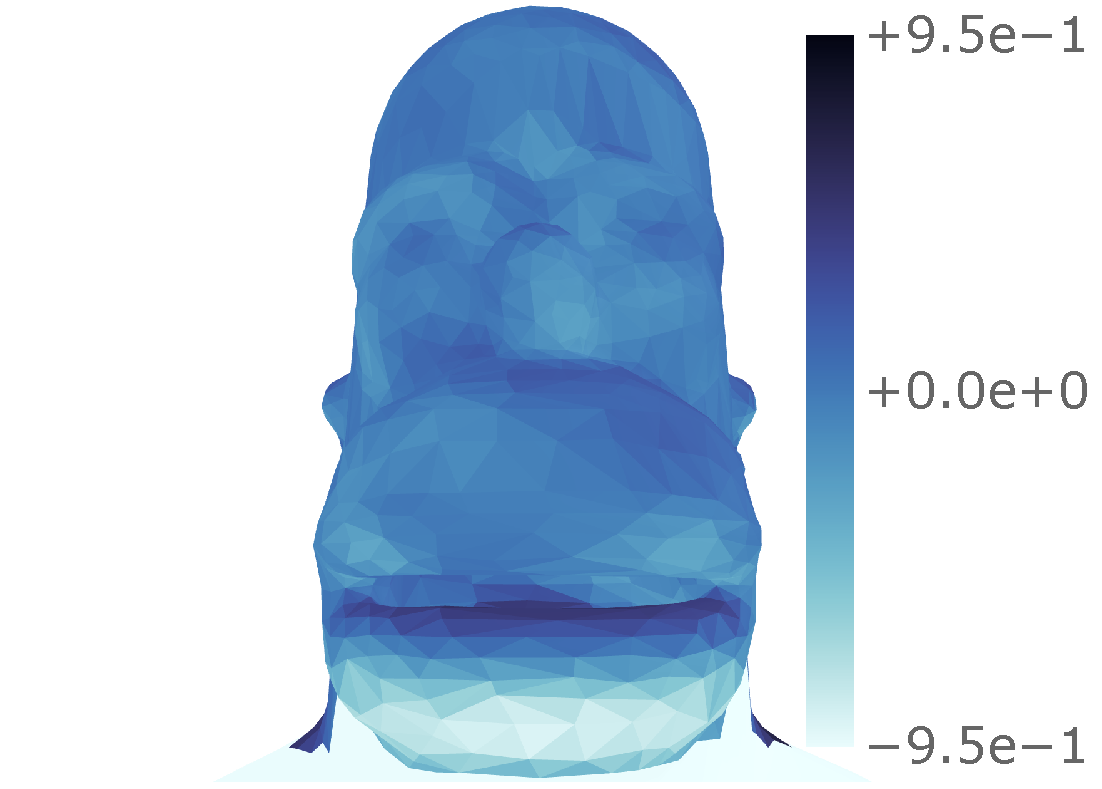
\includegraphics[trim={101 0 3 3},clip,width=.33\textwidth]{slepian_wavelet_coefficients_homer_3B_2jmin_5j_zoom.pdf}}
	\hfill
	\subfloat[\(\mesh{W^{\Psi^{6j}}}\)]
	{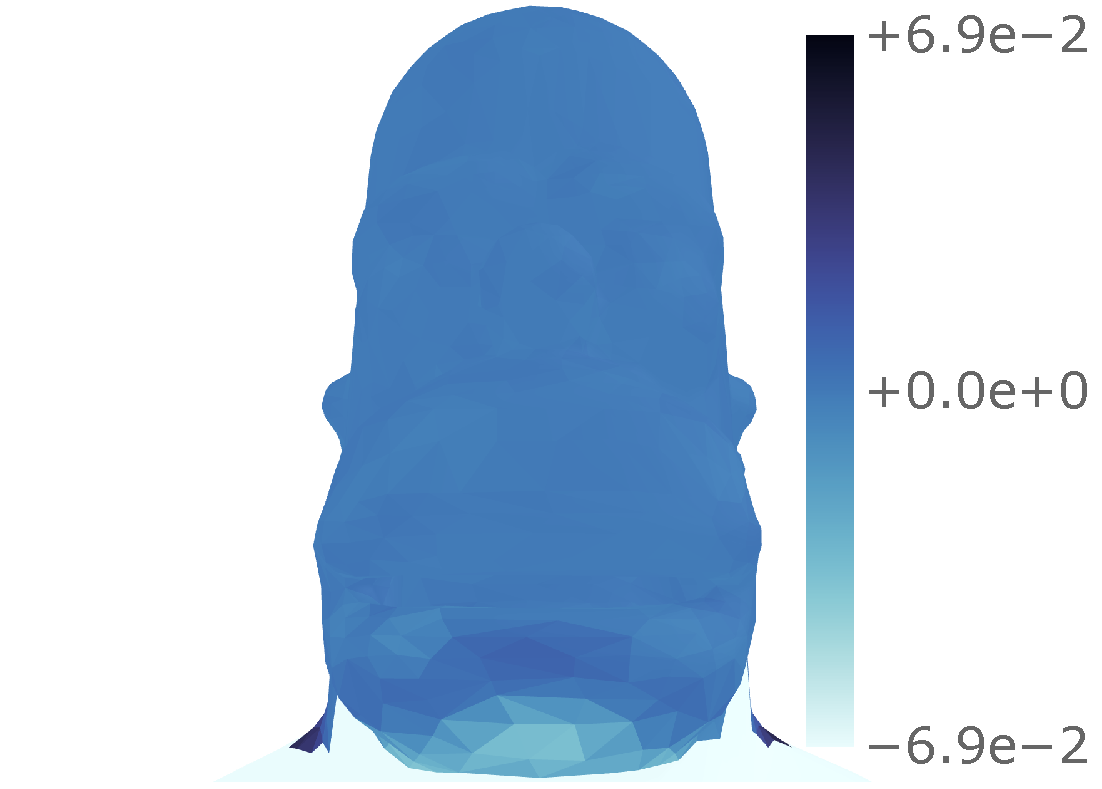
\includegraphics[trim={101 0 3 3},clip,width=.33\textwidth]{slepian_wavelet_coefficients_homer_3B_2jmin_6j_zoom.pdf}}
	\caption{
	}\label{fig:chapter4_wavelet_coefficients}
\end{figure}


\subsection{Wavelet Denoising}\label{sec:chapter4_wavelet_denoising}

Wavelets are used in a variety of contexts in signal processing, one common use case is for denoising a signal.
Localised features in the data can be extracted to different wavelet scales, and hence the desired parts of the signal can be preserved whilst isolating the noise.
To showcase Slepian wavelets, white noise is added to the signal in the right panel of \cref{fig:chapter4_homer_data}.
A straightforward hard-thresholding denoising procedure follows.

Consider a signal localised in the region \(R\) in the presence of noise
%
\begin{equation}\label{eq:chapter4_noised_signal}
	\mesh{z}
	%
	= \mesh{s} + \mesh{n},
\end{equation}
%
where the signal and noise are represented by \(\mesh{s}\) and \(\mesh{n}\) respectively.
The power spectrum of noise in Slepian space is as before
%
\begin{equation}
	\expval{\slepian{n} \conj{\slepian[']{n}}}
	%
	= \sigma^{2} \delta_{pp'}.
\end{equation}
%
To assess the recovery of the initial data, a signal-to-noise ratio for the region is defined
%
\begin{equation}
	\snr{z}
	%
	\equiv 10 \log_{10} \frac{\norm{s}^{2}}{\norm{z - s}^{2}}.
\end{equation}
%
A denoised version of \(z\) is desired, denoted by \(d \in \hilbert{R}\), with a large \(\snr{d}\) such that \(d\) extracts the informative signal \(s\).
Often the scaling coefficients are \emph{not} used in hard-thresholding; however, in the Slepian setting the scaling function and wavelets are treated equivalently.
The scaling function in the Slepian setting is not a low-frequency representation of the signal due to the localisation of the Slepian functions (see \cref{sec:chapter4_localisation}).

Since the wavelet transform is linear, the individual elements sum to give the wavelet/scaling coefficients of \cref{eq:chapter4_noised_signal}
%
\begin{equation}
	\mesh{Z^{\varphi}}
	%
	= \mesh{S^{\varphi}} + \mesh{N^{\varphi}},
\end{equation}
%
where the wavelet coefficients are denoted by capital letters, \ie{}
%
\begin{equation}
	\mesh{Z^{\varphi}} = \mesh{\convolution{\varphi}{z}}.
\end{equation}
%
In wavelet space the noise is
%
%
\begin{equation}
	\variance{\mesh{N^{\varphi}}}
	%
	= \sigma^{2} \slepianSum \abs{\slepian{\varphi}}^{2} \abs{\mesh{\slepian{S}}}^{2}
	%
	\equiv {\mesh{\sigma^{\varphi}}}^{2},
\end{equation}
%
where \(\sigma^{\varphi}\) represents the standard deviation of the noise in wavelet space.
To denoise the signal one may hard-threshold the scaling/wavelet coefficients with a threshold \(T\) proportional to the standard deviation of the noise.
Hence, the denoised wavelet coefficients \(\mesh{D^{\varphi}} = \mesh{\convolution{\varphi}{d}}\) are
%
\begin{equation}
	\mesh{D^{\varphi}} =
	%
	\begin{cases}
		0,
		%
		 & \mesh{Z^{\varphi}} < \mesh{T^{\varphi}},    \\
		%
		\mesh{Z^{\varphi}},
		%
		 & \mesh{X^{\varphi}} \geq \mesh{T^{\varphi}},
	\end{cases}
\end{equation}
%
where
%
\begin{equation}
	\mesh{T^{\varphi}}
	%
	= N_{\sigma}\mesh{\sigma^{\varphi}},
\end{equation}
%
with \(N_{\sigma} \in \realPosParam{}\).
Reconstruction of the signal \(d\) follows by an inverse wavelet transform with these thresholded wavelet coefficients.
This procedure merely demonstrates a practical use case of Slepian wavelets, more sophisticated denoising formalisms can be developed.

To perform the denoising, Gaussian white noise is added to the data in the right panel of \cref{fig:chapter4_homer_data}.
The noised signal is shown in panel (a) of \cref{fig:chapter4_denoising} with an initial signal-to-noise ratio of \(\SI{0.32}{\dB}\).
Panels (b-c) show the results of the denoising procedure describe above for \(N_{\sigma} \in \set{1,2}\), with signal-to-noise ratios of \(\SI{2.29}{\dB}\) and \(\SI{0.98}{\dB}\) respectively.
At \(N_{\sigma}=1\) an initial boost in signal-to-noise ratio is observed; however, as more signal is removed the hard-thresholding scheme experiences diminishing returns.

The same denoising procedure was conducted for a series of other meshes, the Slepian regions of which are shown in \cref{fig:chapter4_other_meshes}.
These meshes are comparable in size to the \(\num{5103}\) vertex Homer mesh, and an appropriate region \(R\) has been highlighted in black for each.
\cref{tab:chapter4_denoising} presents the Shannon number, the number of non-zero wavelets, and the denoising results for each mesh for the same wavelet parameters as before --- \(\lambda=3\) and \(J_{0}=2\).
In general, the hard-thresholding scheme boosts the signal-to-noise ratio of the signal on the mesh, in particular for higher Shannon numbers (more wavelets).
Fine-tuning the wavelet parameters \(\lambda{}\) and \(J_{0}\) would result in a larger signal-to-noise boost for each mesh.

\begin{figure}[htp]
	\centering\capstart{}
	\subfloat[Initial Data]
	{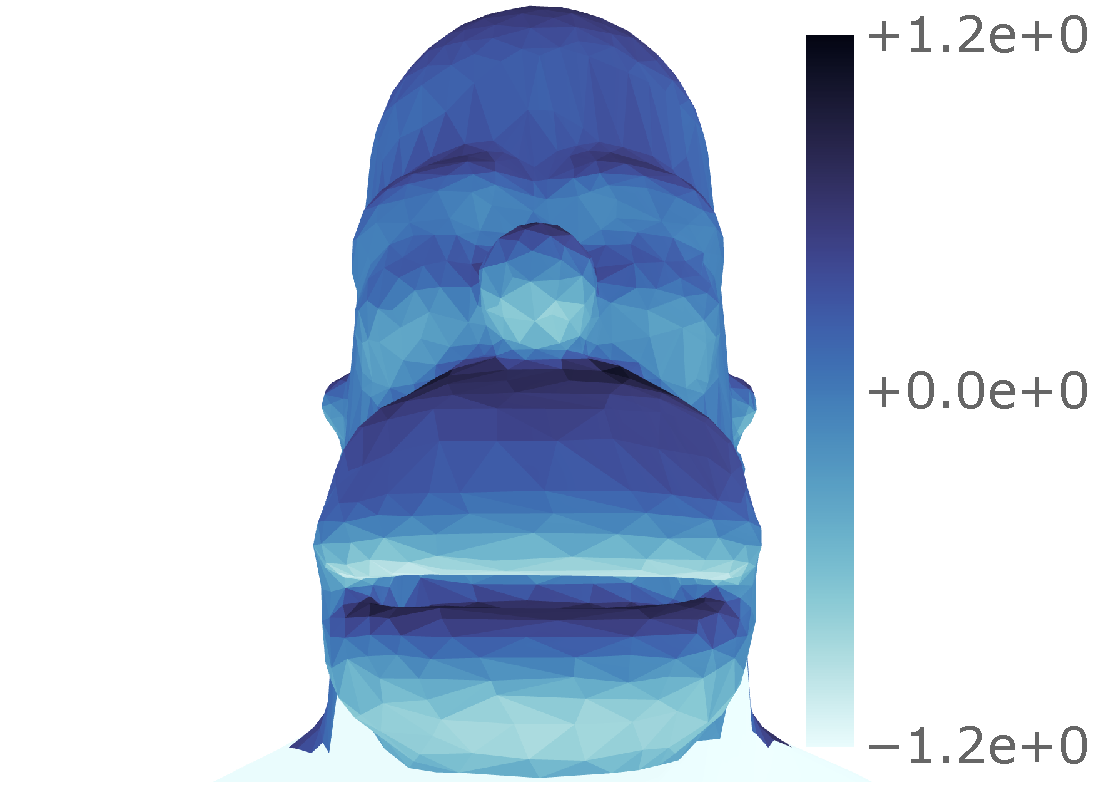
\includegraphics[trim={101 0 3 3},clip,width=.33\textwidth]{slepian_homer_field_zoom.pdf}}
	\hfill
	\subfloat[Noisy Data \newline
		\(\snr{z} = \SI{0.32}{\dB}\)]
	{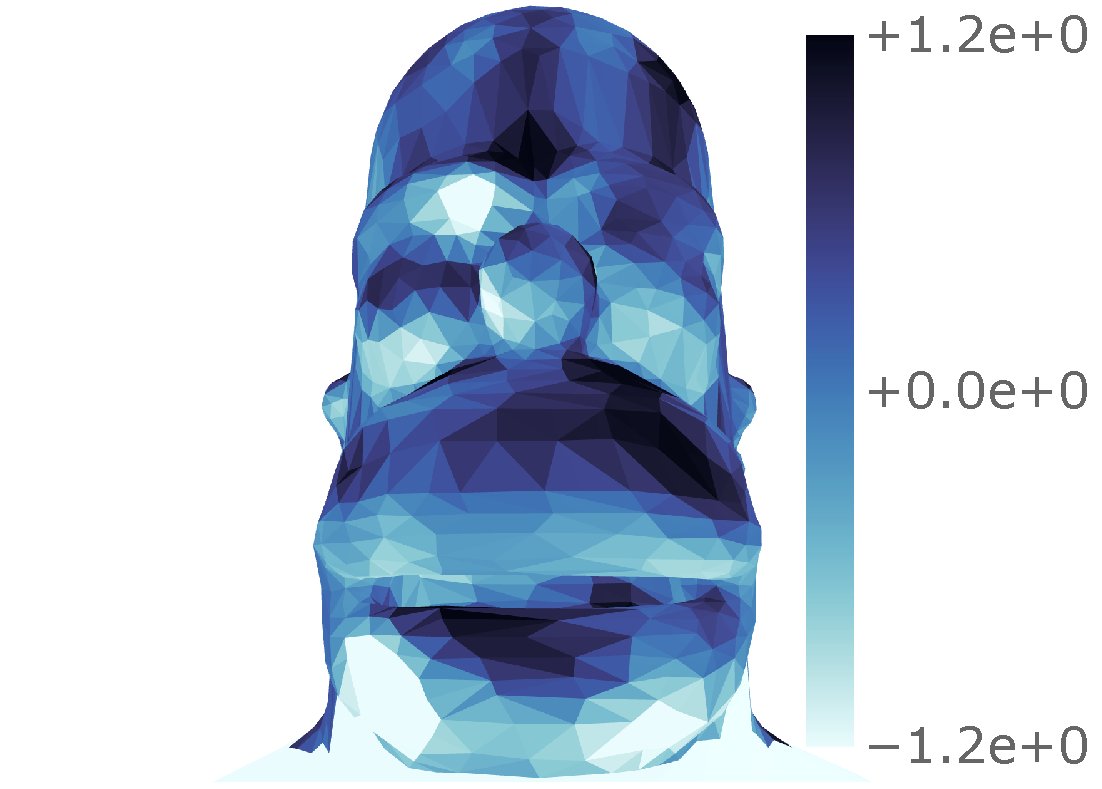
\includegraphics[trim={101 0 3 3},clip,width=.33\textwidth]{slepian_homer_field_-5noise_zoom.pdf}}
	\hfill
	\subfloat[Denoised \(N_{\sigma}=1\) \newline
		\(\snr{d} = \SI{2.29}{\dB}\)]
	{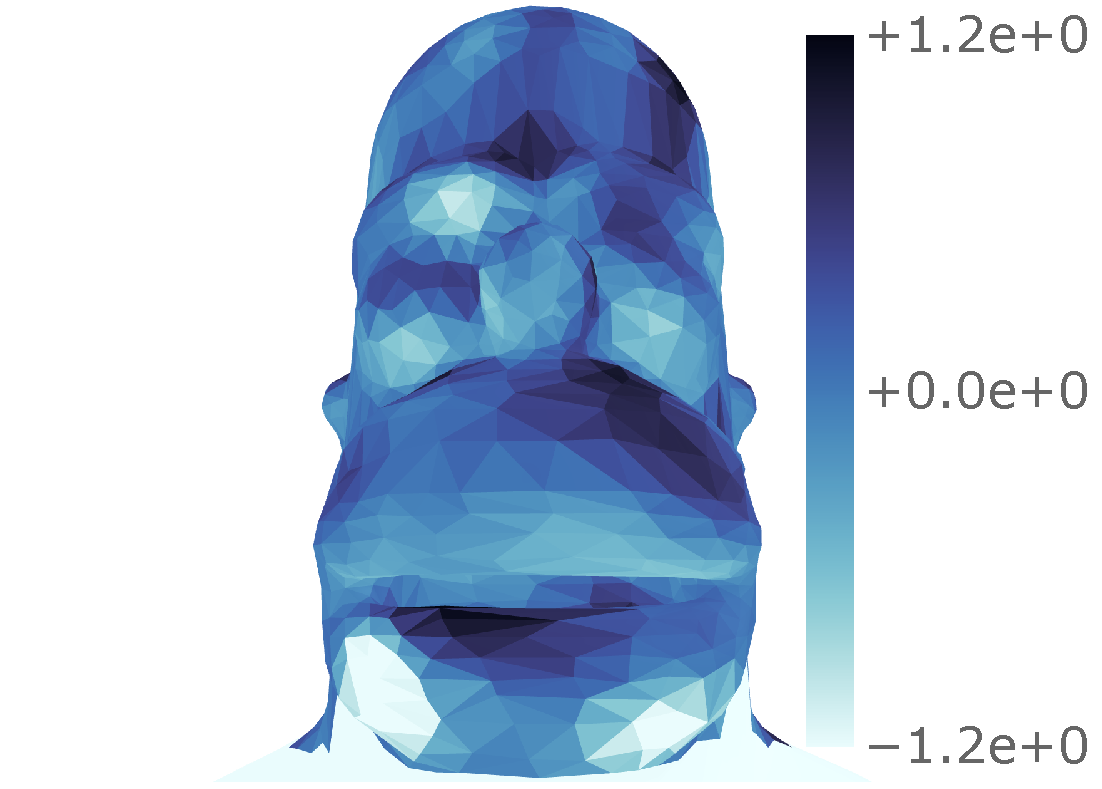
\includegraphics[trim={101 0 3 3},clip,width=.33\textwidth]{homer_-5snr_1n_denoised.pdf}}
	\caption[
		A denoising demonstration for a field on the Homer mesh
	]{
		Panel (a) shows the data in the region \(R\) constructed from the Slepian coefficients of the per vertex normals (\cf{} \cref{fig:chapter4_homer_data}) --- where the field value outside the region is set to negative infinity for illustrative purposes.
		Gaussian white noise is added to the signal in the Homer head region with a signal-to-noise ratio of \(\SI{0.32}{\dB}\), shown in panel (b).
		The scaling and wavelet coefficients of the noisy signal are calculated and are then hard-thresholded with \(N_{\sigma}=1\).
		The corresponding denoised plot is shown in panel (c), where the signal-to-noise ratio is boosted by \(\SI{1.97}{\dB}\) to \(\SI{2.29}{\dB}\).
		Whilst the signal values are defined on the vertices, they have been averaged onto the faces for the plot.
	}\label{fig:chapter4_denoising}
\end{figure}


\begin{figure}[htp]
	\centering
	\subfloat[Bird]
	{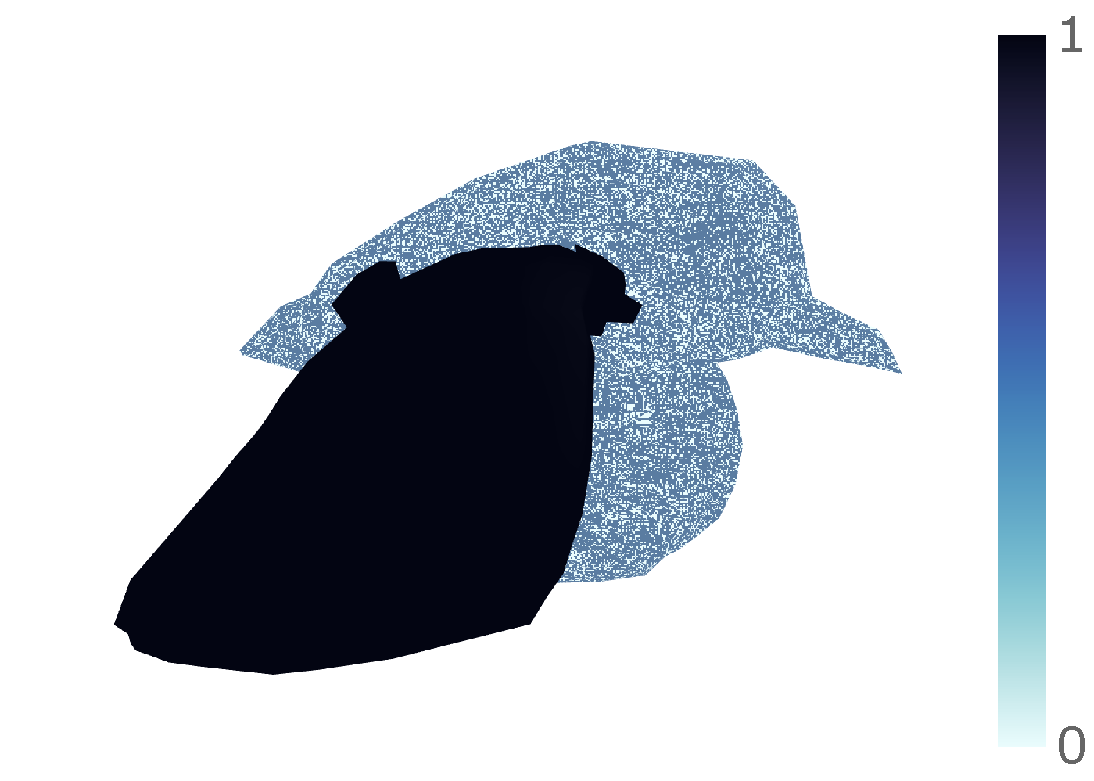
\includegraphics[trim={7 8 3 7},clip,width=.38\textwidth]{bird_region_norm.pdf}}
	\hfill
	\subfloat[Cheetah]
	{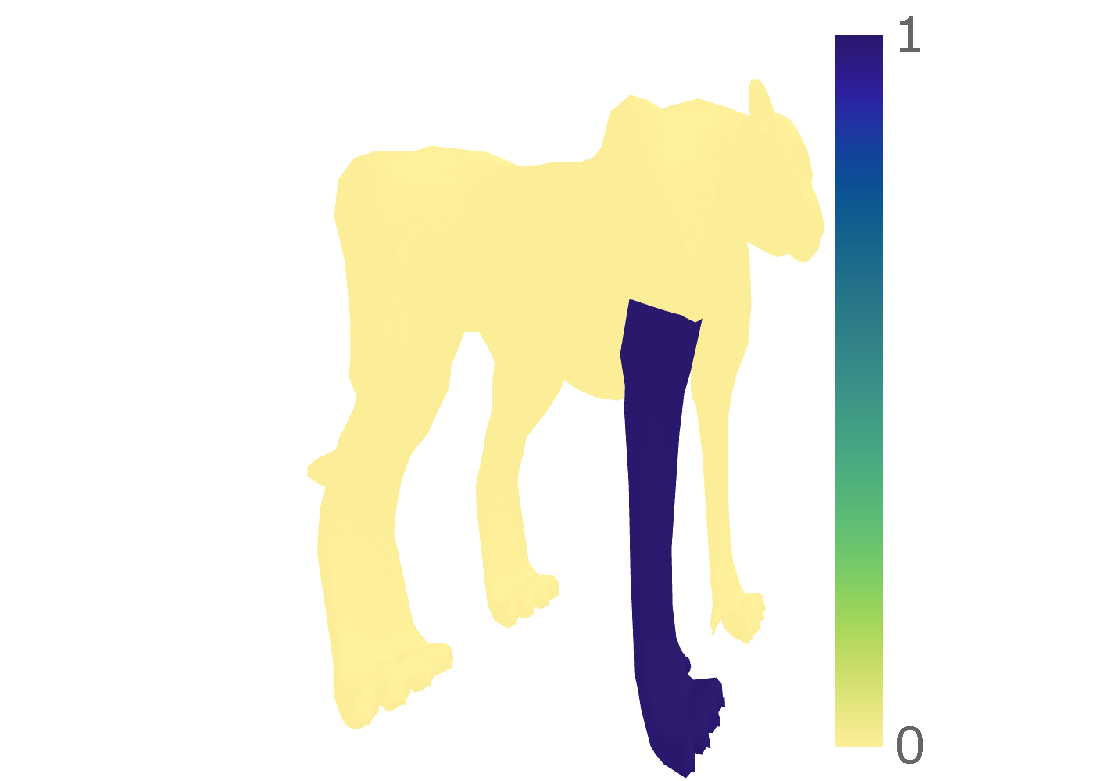
\includegraphics[trim={137 1 3 7},clip,width=.28\textwidth]{cheetah_region_norm.pdf}}
	\hfill
	\subfloat[Cube]
	{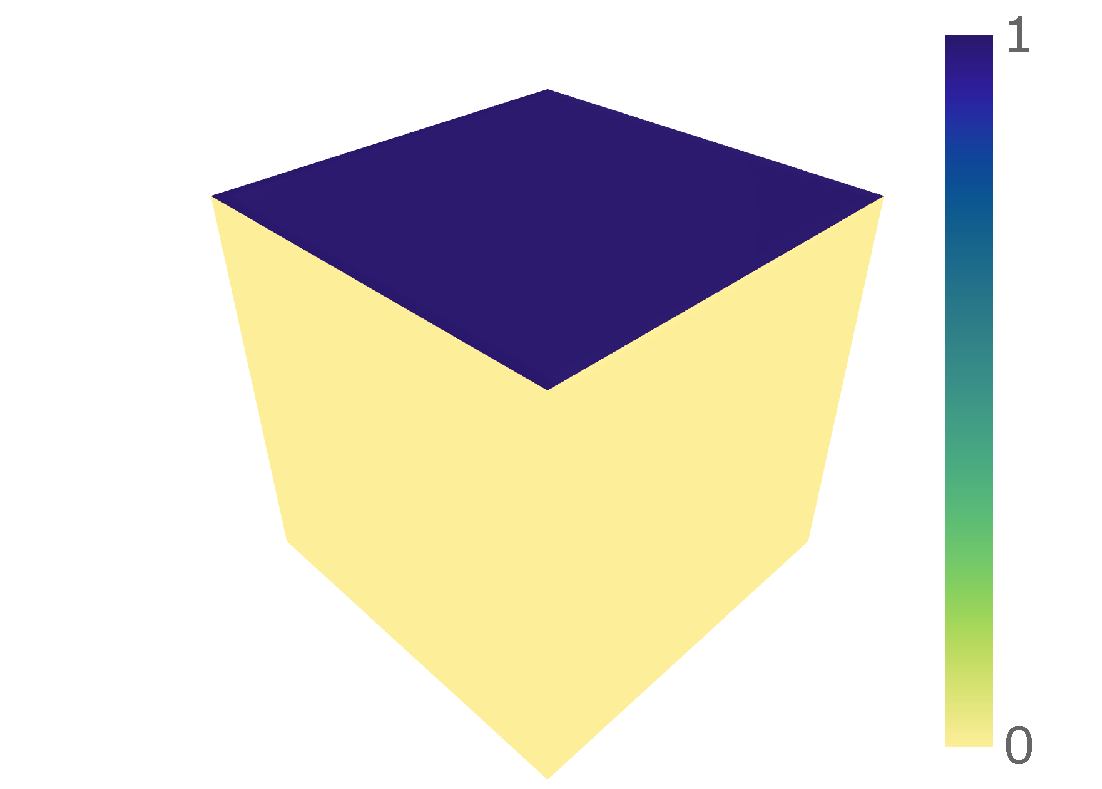
\includegraphics[trim={62 1 3 7},clip,width=.33\textwidth]{cube_region_norm.pdf}}
	\newline
	\subfloat[Dragon]
	{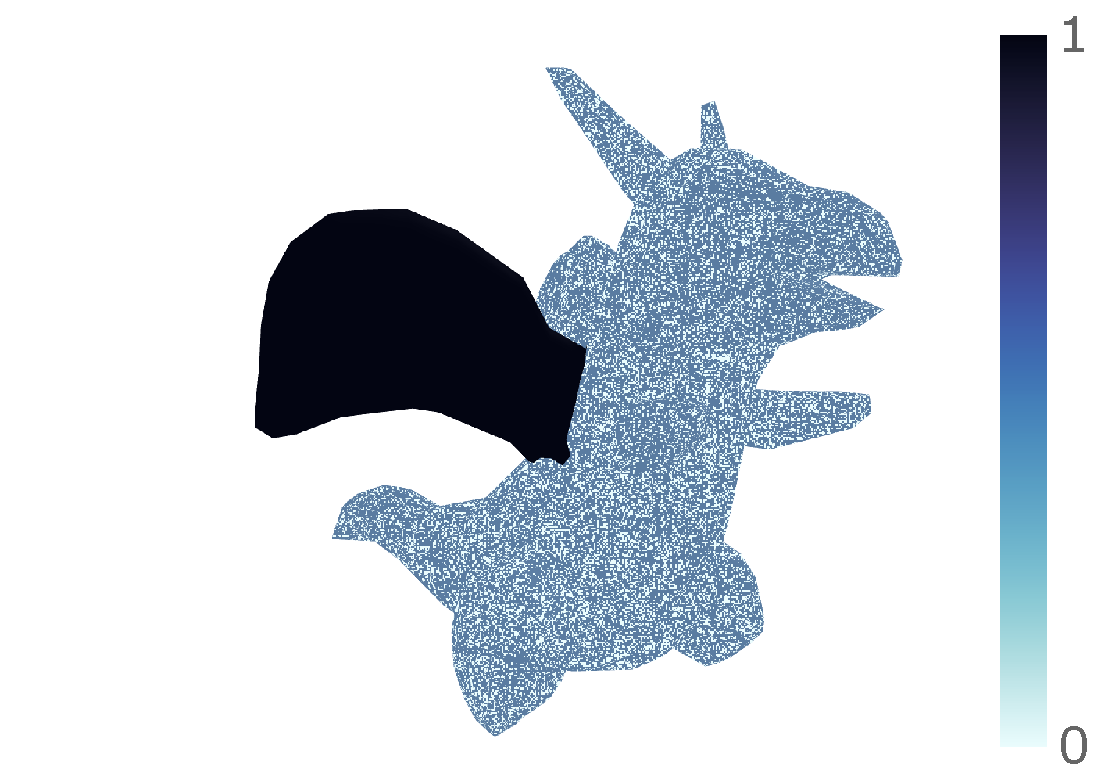
\includegraphics[trim={75 8 3 7},clip,width=.33\textwidth]{dragon_region_norm.pdf}}
	%
	\subfloat[Teapot]
	{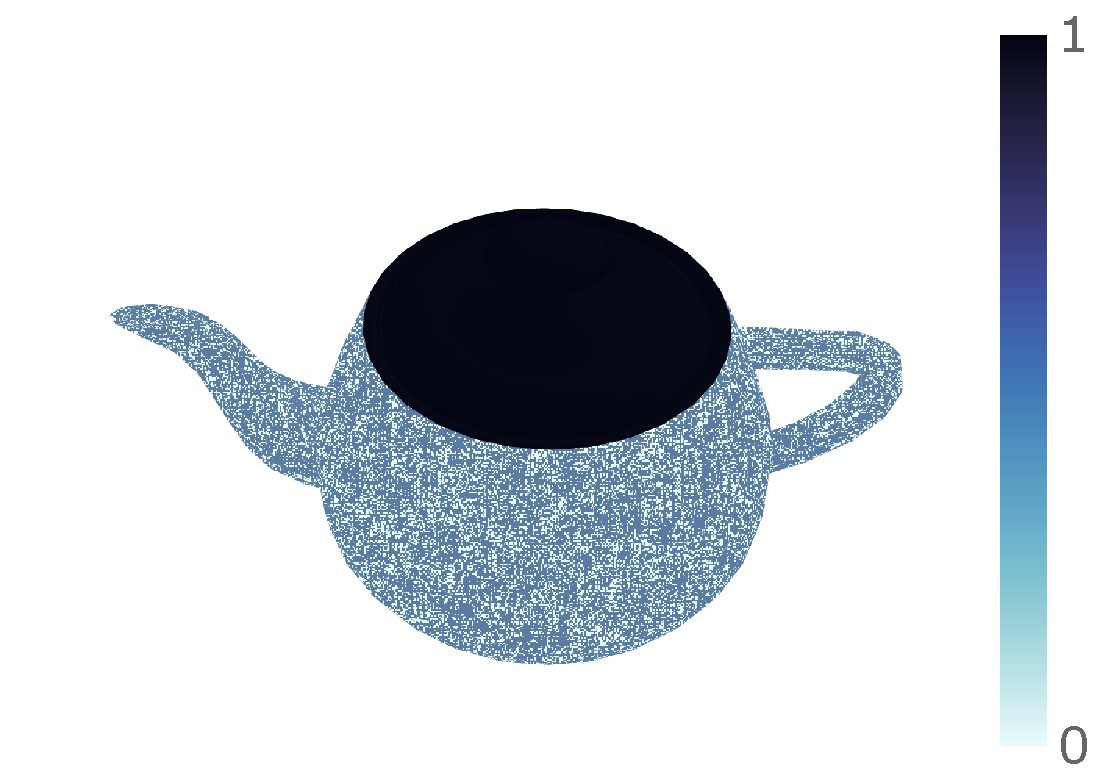
\includegraphics[trim={3 8 3 7},clip,width=.38\textwidth]{teapot_region_norm.pdf}}
	\caption{
		The Slepian regions (in black) of some other meshes.
		The same denoising procedure as in \cref{fig:chapter4_denoising} was performed for these alternative meshes, the results are shown in \cref{tab:chapter4_denoising}.
	}\label{fig:chapter4_other_meshes}
\end{figure}


\begin{table}
	\centering
	\caption{
		Denoising of other meshes.
	}\label{tab:chapter4_denoising}
	\begin{tabular}{@{}rcccc@{}}
		\toprule
		        & Shannon       & Wavelets    & Initial SNR         & \(N_{\sigma}=1\) SNR \\
		\midrule
		Cheetah & \(\num{72}\)  & \(\num{4}\) & \(\SI{3.96}{\dB}\)  & \(\SI{3.58}{\dB}\)   \\
		%
		Dragon  & \(\num{169}\) & \(\num{5}\) & \(\SI{3.44}{\dB}\)  & \(\SI{2.69}{\dB}\)   \\
		%
		Bird    & \(\num{194}\) & \(\num{5}\) & \(\SI{0.49}{\dB}\)  & \(\SI{1.59}{\dB}\)   \\
		%
		Teapot  & \(\num{256}\) & \(\num{6}\) & \(\SI{-1.57}{\dB}\) & \(\SI{-0.08}{\dB}\)  \\
		%
		Cube    & \(\num{272}\) & \(\num{6}\) & \(\SI{2.65}{\dB}\)  & \(\SI{3.85}{\dB}\)   \\
		%
		Homer   & \(\num{329}\) & \(\num{6}\) & \(\SI{0.32}{\dB}\)  & \(\SI{2.29}{\dB}\)   \\
		\bottomrule
	\end{tabular}
\end{table}


\section{Conclusions}\label{sec:chapter4_conclusions}
